\documentclass[11pt]{article}
\usepackage[utf8]{inputenc}
% Style
\usepackage[compilation, transitional, mathfont]{classnotes}

% Figures
\graphicspath{ {/Users/neil/Desktop/PhysicsExamples/} }
\usepackage{chngcntr}
\counterwithin{figure}{section}
\usepackage{float}
\usetikzlibrary{decorations.pathmorphing}
\usepackage{pgfplots}
\pgfplotsset{compat = newest}
\usepgfplotslibrary{colormaps}

% Tables
\usepackage{multirow}

% Make circle (for ammeter/voltmeter)
\newcommand\encircle[1]{
  \tikz[baseline=(X.base)] 
    \node (X) [draw, shape=circle, inner sep=0] {\strut #1};}

\title{AP Physics C: Mechanics}
\author{Neil Rathi}
\date{Semester 1, Fall 2020}

\begin{document}

\maketitle
\noindent These notes are for the first semester of AP Physics C (Mechanics) at Palo Alto High School with Ms. Eris. Since they're typed live during lectures, there will likely be some errors. If you see any, please let me know by emailing me at \href{mailto:neilrathi@gmail.com}{neilrathi@gmail.com} or \href{mailto:neilrathi@gmail.com}{nr26031@pausd.us}.

\setcounter{tocdepth}{1}
\tableofcontents
\newpage

\part{Newtonian Kinematics}
This unit covers unit 1 of the AP Physics C: Mechanics curriculum, as well as a brief introduction to section 2.2.
\section{Motion in One Dimension}
One dimensional motion only considers movement in the $x$ or $y$ axis, with vectors in $\RR^1$.

\subsection{Average Particle Motion}
We start with elementary definitions of displacement, velocity, and acceleration.
\begin{defn}
	Position is the location of a particle with respect to a chosen reference point. Distance is the length of a path followed by a particle, and displacement is an objects change in position. The displacement of a particle with initial position $\vb{x}_i$ and final position $\vb{x}_f$ is
	\[\Delta \vb{x} = \vb{x}_f - \vb{x}_i\]
\end{defn}
Note that displacement is a vector quantity, whereas distance is a scalar quantity. We can also use this to determine the rate of change, or \textit{velocity}, of a particle as defined below.
\begin{defn}[Velocity]
	Average velocity, $\bar{\vb{v}},$ is given by
	\[\bar{\vb{v}} = \frac{\Delta x}{\Delta t} = \vb{v}_{av},\]
	the secant line on a position graph.
\end{defn}
Contrast this with average \textbf{speed}, defined as the total distance over time. Also note that velocity is a vector, notated with boldface or an arrow ($\mathbf{v}$ or $\vec{v}$), whereas speed is a scalar, without an arrow ($v$).

\begin{example}
	Given that the object in the image is moving in a straight line, find the displacement, average velocity, and average speed of the object between A and F.
\end{example}

\begin{figure}[h!t]
	\centering
	\includegraphics[scale=0.4]{phys_notes_ex_one.png}
	\caption{Example 2.1}
\end{figure}

\begin{solution}
	We know that
	\[\Delta \vb{x} = \vb{x}_f - \vb{x}_i = -53 - 30 = \boxed{-83\unt{m}}.\]
	Next, we can calculate that
	\[\vb{v}_{av} = \frac{\Delta \vb{x}}{\Delta t} = -\frac{83}{5} = \boxed{-1.7 \unt{m/s}}.\]	
	Finally,
	\[v_{av} = \frac{\Sigma x}{\Sigma t} = \frac{22 + 105}{50} = \boxed{2.5 \unt{m/s}}.\]
	Note that average velocity and speed are different.
\end{solution}

\subsection{Instantaneous Particle Motion}
As the time interval becomes smaller, average velocity becomes instantaneous, which is the slope of the tangent. Thus,

\begin{defn}[Instantaneous Velocity]
	The instantaneous velocity $\vb{v}$ is
	\[\vb{v} = \lim_{\Delta t \to 0} \frac{\Delta x}{\Delta t} = \dv{x}{t}\]
\end{defn}

\begin{example}
	A particle moves along the $x$ axis according to the expression $x = t^2$. Determine the expression of its instantaneous velocity at any time, and its instantaneous speed at 2s.
\end{example}
\begin{solution}
	We can say that
	\[v(t) = \dv{x}{t} = 2t,\]
	using the power rule. Evaluating this,
	\[\dv{x}{t}\Big|_{t = 2} = \boxed{4 \unt{m/s.}}\]
\end{solution}

\begin{example}
	An object moves according to $x(t) = 2t^3 - t^2 - 4.$ Find the times when it has a velocity of zero.
\end{example}
\begin{solution}
	We can find the velocity function as
	\[v(t) = \dv{t} x(t) = 6t^2 - 2t.\] 
	We set this to zero and get
	\begin{align*}
		6t^2 - 2t &= 0 \\
		2t(3t-1) &= 0 \\
		t &= \boxed{0, \frac{1}{3}}
	\end{align*}
	which is the answer.
\end{solution}

\begin{defn}[Acceleration]
	The average acceleration is the change in velocity over time, given by
	\[\bar{a} = \frac{\Delta \vb{v}}{\Delta t}.\]
	This is also the secant line of the velocity vs. time graph. As intervals get smaller, we find that the instantaneous velocity is
	\[a = \lim_{\Delta t \to 0} \frac{\Delta \vb{v}}{\Delta t} = \dv{v}{t}.\]
	We can also deduce that
	\[a = \dv{t}(\dv{x}{t}) = \dv[2]{x}{t}.\]
\end{defn}

\begin{example}
	An object moves along the x axis according to
	\[x(t) = 3.0t^2-2.0t+3.0\]
	Determine
	\begin{enumerate}
		\item The average speed between 2.0 and 3.0s
		\item The instantaneous speed at 2.0 and 3.0s
		\item The average acceleration between 2.0 and 3.0s
		\item The instantaneous acceleration at 2.0 and 3.0s
	\end{enumerate}
\end{example}
\begin{solution}
	(a) $x(2) = 11,$ $x(3) = 24.$
	\[\bar{\vb{v}} = \frac{\Delta x}{\Delta t} = \frac{13}{1} = \boxed{13 \unt{m/s.}}\]
	(b) $v(t) = \dv{x}{t} = 6t-2$
	\[v(t)\big|_{t=2,3} = \boxed{10, 16 \unt{m/s.}}\]
	(c) $v(2) = 10,$ $v(3) = 16$
	\[\bar{a} = \frac{\Delta v}{\Delta t} = \frac{6}{1} = \boxed{6 \unt{m/s}^2.}\]
	(d) $a = \dv{v}{t} = \dv[2]{x}{t} = \boxed{6 m/s^2}$
\end{solution}

\begin{figure}[h!]
	\centering
	\includegraphics[scale=0.5]{phys_notes_ex_two.png}
	\caption{Various distance, velocity, and acceleration vs. time curves}
\end{figure}

\noindent The slope of the position vs. time gives the velocity, and the slope of velocity gives the acceleration.

\subsection{One Dimensional Motion with Constant Acceleration}
The slope of tangent to displacement gives velocity and slope of velocity gives acceleration.

\begin{eqn}
	The change in velocity is given by
	\[\Delta \vb{v} = at.\]
\end{eqn}
This is the area under the velocity curve.

\begin{eqn}
	The change in displacement is given by
	\[\Delta x = x-x_o = v_ot+\frac{1}{2}at^2\]
\end{eqn}
This is the area under velocity. We can also derive these using the definitions.
Since \[a = \frac{\Delta v}{\Delta t},\]
we have \[v = v_o + at\]
and \[v_{avg} = \frac{v_o + v_f}{2},\]
when acceleration is constant. We also have
\begin{eqn}
The change in displacement is given by
\[x - x_o = \frac{1}{2} (v_o+v)t.\]
\end{eqn}
Thus, we can derive that
\[\Delta x = x-x_o = v_ot+\frac{1}{2}at^2.\]

\begin{eqn}[Timeless Equation]
	For constant $a$,
	\[v^2 = v_0^2 + 2a(x-x_o)\]
\end{eqn}
\begin{proof}
	From equation 2.3, we know
	\[x-x_o = \frac{1}{2}(v_o + v)t.\]
	We can substitute $t$ with $\frac{v-v_o}{a},$ giving us
	\begin{align*}
		x-x_o &= \frac{1}{2}(v_o + v)\left(\frac{v-v_o}{a}\right) \\
		2a(x-x_o) &= (v_o + v)(v-v_o) \\
		2a(x-x_o) &= v^2 - v_o^2 \\
		v^2 &= v_o^2 + 2a(x-x_o),
	\end{align*}
	and we're done.
\end{proof}

\begin{example}
	A car traveling at a constant speed of 45 m/s passes a trooper hidden behind a billboard. One second after the speeding car passes the billboard, the trooper sets out from the billboard to catch it, accelerating at a constant rate of 3.0 m/s$^2$. How long does it tak her to overtake the car?
\end{example}
\begin{solution}
	$v_C = 45.0$ m/s, $a_t = 3.0$ m/s$^2$, $t_{trooper} = t =$ ?, $t_{car} = t+1$. We know that 
	\[\Delta x_{t} = \Delta x_{c},\]
	so we can use 
	\[v_ot+\frac{1}{2}at^2=v_{c}(t+1).\]
	Therefore,
	\[t^2 - 30t - 30 = 0,\]
	so $t = \boxed{31s}$.
\end{solution}

\begin{example}
	A jet lands on an aircraft carrier at 140 mph. (a) What is its acceleration if it stops in 2.0 seconds? (b) If the plane touches down at $x_i = 0,$ what is its final position?
\end{example}
\begin{solution}
	$v_o=63$ m/s, $t = 2.0$ s, $v = 0$, $a = $ ?, $x_o=0$, $x = $ ?.
	(a) We have
	\[a = \frac{v-v_o}{t} = -\frac{63}{2} = \boxed{-31.5\text{m/s}^2}.\]
	(b) We can say
	\begin{align*}
		x-x_i &= \frac{1}{2}(v_o+v)t \\
		x &= \frac{1}{2}(63+0)2 \\
		x &= \boxed{63m},
	\end{align*}
	and we're done.
\end{solution}

\subsection{Free Fall}
Neglecting air resistance, all objects dropped near the surface have the same constant acceleration.
\begin{defn}[Free Fall]
	A \textit{freely falling} object is one that is moving freely under the influence of gravity alone, regardless of its initial motion.
\end{defn}
\begin{example}
	A ball is tossed straight up at 25 m/s. Estimate its velocity at 1s intervals.
\end{example}
\begin{center}
\begin{tabular}{|c|c|}
	\hline
	\textbf{Time} (s) & \textbf{Velocity} (m/s) \\
	\hline
	0 & 25 \\
	\hline
	1 & 15 \\
	\hline
	2 & 5 \\
	\hline
	3 & -5 \\
	\hline
	4 & -15 \\
	\hline
	5 & -25 \\
	\hline
\end{tabular}
\end{center}

\noindent We can apply the same formulas to free fall, setting $a = -g = -9.80$ m/s$^2$.
\begin{eqn}[Free Fall Equations]
	For an object in free fall,
	\[v_y = v_{oy} - gt\]
	\[y-y_o = v_{oy}t - \frac{1}{2}gt^2\]
	\[v_y^2=v_{oy}^2 - 2g(y-y_o)\]
\end{eqn}
In addition, we can determine the vertex points of free fall as follows.
\begin{eqn}[Key Points]
	Where $t_1$ is the vertex point, and $t_2$ is the endpoint of free fall,
	\[t_1 = \frac{v_{oy}}{g}\]
	\[t_2 = 2t_1 = \frac{2v_{oy}}{g}\]
	\[h = \frac{v_{oy}^2}{2g}\]
\end{eqn}

\subsection{Kinematics Equations from Calculus}
We know that the derivative is the instantaneous rate of change. We say that the integral is the antiderivative, or the area under the curve. For some curve $v(t)$,
\[\Delta x = \lim_{n \to \infty}\sum_{i=1}^n v_i\Delta t = \int_{t_i}^t v(t)dt\]
\begin{eqn}
	If $v$ is constant, we have
	\[x - x_o = vt\]
\end{eqn}
\begin{proof}
	We know that
	\[v = \dv{x}{t},\]
	so we can say
	\begin{align*}
	dx &= vdt \\
	\int_{x_o}^{x} dx &= \int_{0}^{t} vdt \\
	x-x_o &= vt,
	\end{align*}
	and we're done.
\end{proof}

\noindent We can also rederive the formula for acceleration. If $a$ is constant,
\begin{align*}
	a &= \dv{v}{t} \\
	dv &= adt \\
	\int_{v_o}^v dv &= \int_{0}^t adt \\
	v - v_{o} &= at
\end{align*}

\section{Vectors}
Vectors are very useful for describing phenomenon in physics. Typically, we work with vectors in $\RR$ and $\RR^2,$ occasionally in $\RR^3,$ and rarely in higher dimensions.
\begin{defn}
	A vector is a quantity with both magnitude and direction.
\end{defn}
\subsection{Basic Vector Operations}
Adding vectors $A$ and $B$ can be done by the tip-to-tail method.
\begin{thrm}[Commutativity]
	Vector sums are commutative. In other words,
	\[\vb{A} + \vb{B} = \vb{B} + \vb{A}.\]
\end{thrm}
\begin{defn}[Negative]
	The negative of a vector $\vb{A}$ is a vector which when added to $\vb{A}$ gives 0.
\end{defn}
When two vectors are subtracted from one another, we draw $-\vb{B},$ and add it to $\vb{A}$.
\begin{thrm}
	When $\vb{A}$ is multiplied by scalar $m,$ the vector $mA$ has the same direction as $A$ and magnitude $mA$.
\end{thrm}
\begin{defn}
	A vector $\vb{A}$ can be expressed as a sum of $A_x$ and $A_y$, where
	\[A_x = A\cos\theta\]
	and
	\[A_y = A\sin\theta.\]
\end{defn}
In Q1, both components are positive. In Q2, the x is negative, and y is positive. In Q3, both are negative, and in Q4, x is positive, and y is negative.

\subsection{Unit Vectors}
We can use unit vectors to express direction and magnitude without specifying the angle of some vector.
\begin{defn}
	A unit vector has magnitude exactly one, and specify a given direction in space. $\vu{i}$ is the $x$ unit vector, $\vu{j}$ is the y unit vector, and $\vu{k}$ is the z unit vector.
\end{defn}
\begin{eqn}
	Since we have
	$$A_x \times \vu{i} = \vb{A}_x\vu{i},$$
	$$A_y \times \vu{j} = \vb{A}_y\vu{j},$$
	$$A_z \times \vu{k} = \vb{A}_z\vu{k},$$
	we can write
	\[\vb{A} = A_x\vu{i}+A_y\vu{j}+A_z\vu{k}.\]
\end{eqn}
\begin{eqn}[Resultant Sum]
	The components of the resultant vector $\vb{R}$ of $\vb{A} + \vb{B}$ are
	\[R_x = A_x + B_x\]
	\[R_y = A_y + B_y\]
	\[R_z = A_z + B_z.\]
\end{eqn}
Since we know
\[R = \sqrt{R_x^2 + R_y^2,}\]
and
\[\tan\theta_R = \frac{R_y}{R_x}\]
we have
\begin{eqn}
	The magnitude of $\vb{R}$ in $\RR^2$ is
	\[|R| = \sqrt{(A_x +B_x)^2 + (A_y + B_y)^2},\]
	and the direction $\theta$ of $\vb{R}$ is given by
	\[\tan\theta = \frac{A_y + B_y}{A_x + B_x}.\]
\end{eqn}
\begin{example}
	Find the magnitude and direction of $10\vu{i} - 6\vu{j}.$
\end{example}
\begin{solution}
	We have that 
	\[|v| = \sqrt{r_x^2 + r_y^2} = \boxed{11.67},\]
	and
	\[\tan\theta = \frac{r_y}{r_x},\]
	so $\theta = \boxed{329^{\circ}}.$
\end{solution}

\subsection{Vector Multiplication}
There are two types of vector multiplication - the dot product and cross product. The dot product gives a scalar, whereas the cross product gives a vector.
\begin{defn}[Dot Product]
	The dot product of $\vb{A}$ and $\vb{B},$ $\vb{A} \cdot \vb{B}$ is a measure of the extent to which the two vectors are in the same direction. This is given by
	\[\vb{A} \cdot \vb{B} = |A||B|\cos\theta.\]
	This is equivalent to
	\[\vb{A}\cdot\vb{B} = (A_xB_x +A_yB_y).\]
\end{defn}
\begin{example}
	Find the angle between
	\[\vb{A} = -7\vu{i} + 4\vu{j}\]
	and
	\[\vb{B} = -2\vu{i}+9\vu{j}.\]
\end{example}
\begin{solution}
	We know that $\vb{A}\cdot\vb{B} = AB\cos\theta.$ We then have that
	\[\vb{A}\cdot\vb{B} = A_xB_x+A_yB_y = 50,\]
	and
	\[A = \sqrt{A_x^2+A_y^2} = 8.06,\]
	\[B = \sqrt{B_x^2+B_y^2} = 9.22,\]
	since $\vb{A}$ and $\vb{B}$ are in $\RR^2.$ Then,
	\[50 = (8.06)(9.22)\cos\theta,\]
	so $\theta = \boxed{47.7^{\circ}}.$
\end{solution}
\begin{defn}[Cross Product]
	The cross product of vectors $\vb{A}$ and $\vb{B}$ is
	\[\vb{A} \times \vb{B} = \vb{C} = AB\sin\theta,\]
	where $\vb{C}$ is the normal vector to $\vb{A}$ and $\vb{B}$.
\end{defn}
We can use the right hand rule to determine the direction of $\vb{C}.$ This also indicates that $\vb{C}$ must be in $\RR^3.$ The commutative law does not hold with cross products.
\begin{example}
	Vector $\vb{A}$ is in $\RR^2,$ along $x-y$, and has a magnitude of 18 units, pointing in a direction $250^{\circ}$ from the x axis. Vector $\vb{B}$ has magnitude 12, and points along $z$. What is $\vb{A}\times\vb{B}$?
\end{example}
\begin{solution}
	We can write $\vb{A}$ and $\vb{B}$ as
	\[\vb{A} = A_x\vu{i} + A_y\vu{j}\]
	and
	\[\vb{B} = B_z\vu{k},\]
	respectively. Then,
	\begin{align*}
		\vb{C} &= \vb{A} \times \vb{B} \\
		&= (A_x\vu{i} + A_y\vu{j}) \times (B_z\vu{k}) \\
		&= A_xB_z(\vu{I}\times\vu{k}) + A_yB_z(\vu{j}\times\vu{k}) \\
		&= A_xB_z(-\vu{j}) + A_yB_z(\vu{i}) \\
		&= -202.9\vu{i}+73.9\vu{j},
	\end{align*}
	and we're done.
\end{solution}

\section{Two Dimensional Kinematics}
Currently, we've been describing motion with one-dimensional objects (that is, vectors in $\RR$). However, most objects follow trajectories more accurately described in $\RR^2$.
\subsection{Analyzing 2D Motion}
To precisely describe motion in two dimensions, we use the position vector $\vec{r}.$
\begin{eqn}
	Given two position vectors $\vec{r}_{t_1}$ and $\vec{r}_{t_2}$ at times $t_1$ and $t_2$ on a motion graph, the displacement, $\Delta \vec{r}$ is given by
	\[\Delta \vec{r} = \vec{r}_{t_2} - \vec{r}_{t_1}\]
\end{eqn}
In addition, we know that $\vec{v}_av = \frac{\Delta \vec{r}}{\Delta t}$. This means that
\begin{eqn}
	For displacement $\Delta \vec{r}$ and time $\Delta t,$
	\[\vec{v} = \dv{\vec{r}}{t} = \dv{x}{t} \vu{i} + \dv{y}{t}\vu{j}.\]
	In addition, we have
	\[\vec{a} = \dv{\vec{v}}{t} = \dv[2]{\vec{r}}{t}\]
\end{eqn}

\begin{example}
	An object is described by the position
	\[\vec{r}(t) = (3t^3-4t)\vu{i} + (1-\frac{1}{2}t^2)\vu{j}.\]
	Find its velocity and position for arbitrary times.
\end{example}
\begin{solution}
	From Equation 1.1, we know that velocity is the derivative of position with respect to time. Therefore,
	\begin{align*}
		\vec{v}(t) &= \dv{\vec{r}}{t} \\
		&= \dv{x}{t}\vu{i} + \dv{y}{t}\vu{j} \\
		&= \boxed{(9t^2-4)\vu{i}-(t)\vu{j}}.
	\end{align*}
	We also have that acceleration is the derivative of velocity, so
	\begin{align*}
		\vec{a}(t) &= \dv{\vec{v}}{t} \\
		&= \boxed{18t\vu{i} - 1\vu{j}},
	\end{align*}
	and we're done.
\end{solution}

\subsection{Analyzing Projectile Motion}
In projectile motion, the velocity vector can be described as two independent component vectors, $\vec{v}_x$ and $\vec{v}_y$. The $x$ component has constant velocity, and the $y$ component has constant acceleration ($-g$).
\begin{eqn}
	With initial velocity $v_0$ and initial angle $\theta$,
	\[v_{0x} = v_0\cos\theta\]
	\[v_{0y} = v_0\sin\theta.\]
\end{eqn}
Horizontal and vertical motion are independent, so we can analyze them separately.
\begin{eqn}[Horizontal Motion Equations]
	Since the $x$ component has constant velocity,
	\begin{align*}
		v_x &= v_{ox} \\
		\Delta x &= v_{ox}t.
	\end{align*}
\end{eqn}
\begin{eqn}[Vertical Motion Equations]
	Since the $y$ component has constant acceleration,
	\begin{align*}
		v_y &= v_{oy} - gt \\
		\Delta y &= \frac{1}{2}(v_y + v_{oy})t \\
		\Delta y &= v_{oy}t - \frac{1}{2}gt^2 \\
		v_y^2 &= v_{oy}^2 - 2g\Delta y
	\end{align*}
\end{eqn}
\begin{remark}
	A positive velocity is upwards and towards the right.
\end{remark}
\begin{example}
	A ball rolls off a table 1.0 m high with a speed of 4 m/s. How far from the base does it land?
\end{example}
\begin{solution}
	We know $\Delta y = -$1.0 m, $v_{ox} =$ 4 m/s, and $v_{oy} = 0$. Thus,
	\begin{align*}
		\Delta y &= v_{oy}t - \frac{1}{2}gt^2 \\
		-1 &= - \frac{1}{2}(9.8)t^2 \\
		t &= -0.45s.
	\end{align*}
	Then, we can say
	\begin{align*}
		\Delta x &= v_{ox}t \\
		&= \boxed{1.8\unt{m}},
	\end{align*}
	and we're done.
\end{solution}
\begin{thrm}
	The trajectory of a projectile is parabolic, given by
	\[y = \left(\frac{v_{oy}}{v_{ox}}\right)x + \left(-\frac{g}{2v_{ox}}\right)x^2.\]
\end{thrm}
\begin{proof}
	We can say that
	\[t = \frac{\Delta x}{v_{ox}},\]
	from 2.2. We also know that
	\[\Delta y = v_{oy}t - \frac{1}{2}gt^2,\]
	from 2.3. Substituting $t$ with $\frac{\Delta x}{v_{ox}},$ we get
	\[\Delta y = v_{oy}\left(\frac{\Delta x}{v_{ox}}\right) - \frac{1}{2}g\left(\frac{\Delta x}{v_{ox}}\right)^2,\]
	so
	\[y = \left(\frac{v_{oy}}{v_{ox}}\right)x^2 - \left(\frac{g}{2v_{ox}^2}\right)x^2,\]
	which was to be proved.
\end{proof}
\begin{eqn}
	The maximum height and range of a projectile are
	\[h = \frac{v_{o}^2\sin^2\theta}{2g}\]
	and
	\[R = \frac{v_o^2\sin2\theta}{g}.\]
\end{eqn}
\begin{proof}
	For the height, we know that $v_y = 0$ at the maximum height. Thus,
	\[v_o\sin\theta-gt = 0,\]
	since $v_{oy} = v_o\sin\theta$. Therefore,
	\[t_h = \frac{v_o\sin\theta}{g}.\]
	We can then substitute into $\Delta y = v_{oy}t - \frac{1}{2}gt^2,$ so it becomes
	\[h = (v_o\sin\theta)\frac{v_o\sin\theta}{g}-\frac{1}{2}g\left(\frac{v_o\sin\theta}{g}\right)^2.\]
	From basic algebra,
	\begin{align*}
		h &= \frac{v_o^2\sin^2\theta}{g} - \frac{g}{2}\left(\frac{v_o\sin\theta}{g}\right)^2 \\
		&= \frac{v_o^2\sin^2\theta}{g} - \frac{g}{2}\cdot\frac{v_o^2\sin^2\theta}{g^2} \\
		&= \frac{v_o^2\sin^2\theta}{g} - \frac{v_o^2\sin^2\theta}{2g} \\
		&= \frac{2v_o^2\sin^2\theta - v_o^2\sin^2\theta}{2g} \\
		&= \frac{v_{o}^2\sin^2\theta}{2g},
	\end{align*}
	and we're done. For the range, we know $R = v_{ox}t.$ Therefore,
	\[R = v_o\cos\theta\cdot 2t_h,\]
	since the distance is reached after twice the time it takes to reach the maximum height. From earlier, we have
	\[t_h = \frac{v_o\sin\theta}{g},\]
	so substituting,
	\[R = v_o\cos\theta\cdot \frac{2v_o\sin\theta}{g}.\]
	We also know that $2\sin\theta\cos\theta = \sin2\theta.$ Therefore,
	\[R = \frac{v_o\sin2\theta}{g},\]
	which was to be proved.
\end{proof}
\begin{example}
	An arrow is shot from a castle wall 10.0 m high. It leaves the bow with speed 40.0 m/s directed 37$^{\circ}$ above the horizontal. Find the initial velocity components and the maximum height of the arrow.
\end{example}
\begin{solution}
	For part (a), we have
	\[v_{ox} = v_o\cos\theta = 32 m/s\]
	\[v_{oy} = v_{o}\sin\theta = 24 m/s.\]
	For part (b), we can use 2.5, so
	\[h = \frac{40^{2}\left(\sin\left(37\right)\right)^{2}}{9.8\cdot2}+10 = \boxed{39.56 m},\]
	and we're done.
\end{solution}

\section{Circular Motion}
Motion isn't just constrained rectilinearly--we can also describe the motion of a particle in circular orbit.
\subsection{Particle in Uniform Circular Motion}
An object moving in a circular path is said to be in circular motion if it has constant speed. However, the velocity changes in direction. Therefore, the object is accelerating.

\begin{thrm}
	The direction of $\Delta v$ is towards the center of the circular path.
\end{thrm}
Since the magnitude of velocity is constant, the acceleration vector can only have a component perpendicular to path.
\begin{eqn}
	The centripetal acceleration (center-seeking) $a_c$ is given by
	\[a_c = \frac{v^2}{r}\]
\end{eqn}
\begin{proof}
	From similar triangles, we know that
	\[\frac{\Delta \vb{r}}{\vb{r}} = \frac{\Delta \vb{v}}{\vb{v}},\]
	where $\vb{r}$ is the position vector. Therefore,
	\[\Delta v = \frac{v\Delta r}{r}.\]
	We also know that
	\[\vb{a} = \frac{\Delta \vb{v}}{\Delta t}.\]
	Substituting,
	\begin{align*}
		\vb{a} &= \frac{\frac{\vb{v}\Delta \vb{r}}{\vb{r}}}{\Delta t} \\
		&= \frac{\vb{v}^2}{\vb{r},}
	\end{align*}
	since $\vb{r}/t = \bar{\vb{v}}$, and $\bar{\vb{v}}$ is the same as $\vb{v}$ (because velocity is constant). Thus, we are done.
\end{proof}

\begin{defn}[Period]
	The period, $T$ is the time required for one complete revolution. It is given by
	\[T = \frac{2\pi r}{v}.\]
\end{defn}
This also lets us derive
\begin{eqn}[Tangential Velocity]
	The tangential velocity is given by
	\[\vb{v} = \frac{2\pi r}{T}.\]
\end{eqn}
This is easily derived from Definition 1.1.
\begin{defn}[Angular Motion]
	Angular displacement, $\theta$ is parallel to displacement, $x$. Angular velocity, $\omega$, is parallel to velocity $\vb{v}$, and angular acceleration, $\alpha$, is parallel to linear acceleration $\vb{a}$.
\end{defn}
\begin{eqn}
	The angular velocity, $\omega$ is given by angular displacement over time:
	\[\omega = \frac{\theta}{t}.\]
	For one revolution,
	\[\omega = \frac{2\pi}{T},\]
	since $\theta = 2\pi$ in one revolution.
\end{eqn}
\begin{eqn}
	Tangential velocity, $\vb{v}$ is given as
	\[v = r\omega,\]
	or \textit{romega}.
\end{eqn}

\subsection{Tangential and Radial Acceleration}
When speed and direction change, acceleration has a tangential and radial component (such as in a roller coaster). We write $a_r$ for radial, which indicates that the object turns, and $a_t$ for tangential, which indicates that the object speeds up.
\begin{eqn}
	The components of $\vb{a}$ are given by
	\[a_t = \dv{v}{t}\]
	and
	\[a_r = \frac{v^2}{r}\]
\end{eqn}
\begin{remark}
	Centripetal acceleration is the same as radial acceleration, and we use $a_c$ when there is no tangential acceleration.
\end{remark}
Since we have the perpendicular components, we can say
\begin{eqn}
	The magnitude of $\vb{a}$ is
	\[|\vb{a}| = \sqrt{(a_r)^2+(a_t)^2}.\]
\end{eqn}
\begin{proof}
	This is a result of the Pythagorean Theorem.
\end{proof}

\begin{example}
	The diagram represents the total acceleration of a particle moving clockwise in a circle of radius $2.50$ m at a certain instant of time. At this instant, find the radial acceleration, the speed of the particle, and the tangential acceleration.
\end{example}
\begin{solution}
	$a = 15.0$ m/s$^2$ at $30.0^{\circ}$, and r = 2.50 m. We know that
	\[a_r = a\cos 30^{\circ} = \boxed{13.0 \unt{m/s}^2},\]
	from trig. Then, we have
	\begin{align}
		a_r &= \frac{v^2}{r} \\
		v &= \sqrt{a_r \cdot r} \\
		&= \boxed{5.7 \unt{m/s}}.
	\end{align}
	Finally,
	\[a_t = 15\sin30^{\circ} = \boxed{7.5 \unt{m/s}^2},\]
	and we're done.
\end{solution}

\subsection{Relative Motion}
Relative motion studies how different observers may interpret motion differently based on their vantage point.
\begin{example}
Suppose a bus is moving to the right with a speed of 15 m/s, and a passenger walks to the front of the bus with 2 m/s. What is the speed of the passenger as observed from the side of the road?
\end{example}
\begin{solution}
	$\vec{v}_{BG} = 15$ m/s, right, and $\vec{v}_{PB} = 2$ m/s, right. We want to find $\vec{v}_{PG}.$ We can use vector addition, which says
	\[\vec{v}_{PB} + \vec{v}_{BG} = \vec{v}_{PG},\]
	from the tip to tail method. Thus,
	\[\vec{v}_{PG} = 15 + 2 = \boxed{17 \unt{m/s}},\]
	and we're done.
\end{solution}

\begin{example}
	A slower car with a speed of 12 m/s is traveling behind a faster bus with a speed of 16 m/s. A passenger on the bus gets up and walks toward the front of the bus with a speed of 2 m/s. What is the velocity of the passenger relative to the car?
\end{example}
\begin{solution}
	We have $\vec{v}_{CG} = 12$ m/s, $\vec{v}_{BG} = 16$ m/s, $\vec{v}_{PB} = 2$ m/s. We want to find $\vec{v}_{PC},$ so we can use the tip to tail method:
	\[\vec{v}_{PC} = \vec{v}_{P\phantom{A}} + \vec{v}_{\phantom{AA}} + \vec{v}_{\phantom{A}C}.\]
	We then have that
	\[\vec{v}_{PC} = \vec{v}_{PB} + \vec{v}_{BG} + \vec{v}_{GC}.\]
	Since $\vec{v}_{GC} = -\vec{v}_{CG},$
	\[\vec{v}_{PC} = 2 + 16 - 12,\]
	so we have $\vec{v}_{PC} = \boxed{+6 \unt{m/s}}.$
\end{solution}

\begin{example}
	A small aircraft is heading south with a speed of 57.8 m/s with respect to still air. Suddenly, a wind blows the plane so it moves in a direction 45$^{\circ}$ west of south with 90.0 m/s with respect to the ground. Determine the velocity of the wind with respect to the ground.
\end{example}
\begin{solution}
	We know $\vec{v}_{PA} = 57.8$ m/s, S, $\vec{v}_{PG} = 90.0$ m/s, 45$^{\circ}$ W of S. We want to find $\vec{v}_{AG},$ so from the bookend method,
	\begin{align*}
		\vec{v}_{AG} &= \vec{v}_{A\phantom{P}} + \vec{v}_{\phantom{P}G} \\
		&= \vec{v}_{AP} + \vec{v}_{PG}.
	\end{align*}
	Since we have $\vec{v}_{AP} = -\vec{v}_{PA} = 57.8$ m/s, N. Geometrically, we can't use the pythagorean theorem, so we can instead find the components and add. We need $\vec{v}_{PGx}, \vec{v}_{PGy}, \vec{v}_{APx},$ and $\vec{v}_{APy}$. We also know that $\vec{v}_{APx} = 0$. We have
	\[\vec{v}_{PGx} = 90\cos45, W,\]
	\[\vec{v}_{PGy} = 90\sin45, S,\]
	\[\vec{v}_{APy} = 57.8, N.\]
	Let South be positive, and north be negative. Then,
	\[\vec{v}_{AGx} = 63.6, W\]
	and
	\[\vec{v}_{ABy} = 5.8, S.\]
	Thus,
	\[\vec{v}_{AG} = \sqrt{63.6^2 + 5.8^2} = 63.9 \unt{m/s.}\]
	We can then say that
	\[\theta = \tan^{-1}\left(\frac{63.6}{5.8}\right) \approx 85^{\circ}.\]
	Therefore, $\vec{v}_{AF} = 63.9\unt{m/s at }85^{\circ}\unt{West of South}$.
\end{solution}

\newpage

\part{Forces}
This unit covers unit 2 of the AP Physics C: Mechanics curriculum.
\section{Introduction to Forces}
There are two types of forces: contact and non-contact. For example, contact forces include
\begin{enumerate}
	\item Pushing and Pulling ($F$)
	\item Tension ($T$)
	\item Surface
		\begin{enumerate}
			\item Normal ($n$ or $F_N$)
			\item Friction ($f_s$ and $f_k$)
		\end{enumerate}
\end{enumerate}
Non-contact forces include
\begin{enumerate}
	\item Gravity ($F_g = mg$)
	\item Electric ($F_e$)
	\item Magnetic ($F_b$)
\end{enumerate}
Free body diagrams show the relative magnitude and direction fo all forces acting upon an object in a given situation. When drawing free body diagrams,
\begin{enumerate}
	\item Identify which forces are present
	\item Determine the direction in which each force is acting
	\item Draw a box to represent the object, and arrows to represent each force
	\item Label each force arrow according to its type
\end{enumerate}
\begin{example}
	Two blocks, A and B, are pulled up on an inclined plane as shown in the diagram. The blocks do not slip against each other. Draw a free body diagram for each block.
\end{example}

\begin{solution}
The force of gravity pulls downwards, and there is a normal force between the two blocks. In addition, there is a tension force on A, and friction between them (and between B and the plane). Therefore, we have
\begin{figure}[h!]
	\centering
	\includegraphics[scale=0.4]{force_notes_ex1.png}
	\caption{Example 3.1}
\end{figure}

\noindent and we're done.
\end{solution}

\subsection{Newton's First Law}
Newton's first law gives us the concept of inertia, which is used to define mass.
\begin{law}[First Law of Motion]
	An object at rest will remain at rest, or if in uniform motion it will continue as such, unless acted upon by a net (unbalanced) external force.
\end{law}
\begin{defn}[Inertia]
	The inertia of an object is its tendency to resist any attempt to change its velocity.
\end{defn}
Internal forces cannot change an objects motion.
\subsection{Mass}
An object which uniformly moves and an object at rest both have the same inertia. This is because of the definition of mass.
\begin{defn}[Mass]
	Mass is a measure of resistance an object exhibits to changes in its velocity. The more massive an object is, the more inertia it has. Mass is a scalar, measured by the SI unit of kilograms (kg).
\end{defn}
Mass differs from weight in that it is independent of the objects surroundings and of the method used to measure it.
\subsection{Newton's Second Law}
Newton's second law answers the question of a nonzero resultant/net force acting on an object.
\begin{law}[Second Law of Motion]
	The magnitude of the acceleration of an object is inversely proportional to its mass. That is,
	\[a = \frac{\Sigma F}{m}.\]
\end{law}
Force is measured in Newtons (N), where 1 newton is the force that produces an acceleration of 1 m/s$^2$ when acting on a 1 kg mass.
\begin{eqn}
	A newton is defined as
	\[1 N = 1 kg \cdot m/s^2\]
\end{eqn}
\begin{example}
	A hockey puck with a mass of 0.30 kg slides on the horizontal frictionless surface of an ice rink. Two hockey sticks strike the puck simultaneously, exerting the forces on the puck shown below.
	\begin{enumerate}
		\item Determine both the magnitude and direction of the puck's acceleration
		\item Suppose a third hockey stick strikes the puck simultaneously with the other two. The puck shows no acceleration. What must be the components of the third force?
	\end{enumerate}
\end{example}
\begin{figure}[h!]
	\centering
	\includegraphics[scale=0.4]{force_notes_ex2.png}
	\caption{Example 3.2}
\end{figure}

\begin{solution}
	The diagram shows
	We can say that
	\[\Sigma F_{x} = F_{1x} + F_{2x} = 5\cos20+8\cos60 = 8.967 N\]
	and
	\[\Sigma F_{y} = F_{1y} + F_{2y} = 5\sin20+8\sin60 = 5.217 N.\]
	Then, since
	\[\Sigma F = \sqrt{F_{x}^2 + F_{y}^2},\]
	we have $\Sigma F = 10.142 N,$ so then
	\[a = \frac{\Sigma F}{m} = 34\unt{m/s}^2.\]
	Using trig, we have
	\[\theta = \tan^{-1}\left(\frac{5.217}{8.697}\right) = 31^{\circ}.\]
	For part b, we now have
	\[F_3 = -\Sigma F_{x}\vu{i} - \Sigma F_{y}\vu{j},\]
	so $\boxed{F_{3} = -8.7\vu{i} - 5.2\vu{j} N}.$
\end{solution}

\subsection{Gravitational Force and Weight}
A mass in free fall experiences the force of gravity. From Newton's Second Law, we can derive
\begin{eqn}
	The force of gravity on an object is
	\[F_g = mg,\]
	where $m$ is its mass and $g$ is the acceleration due to gravity.
\end{eqn}
Therefore, mass is universal, but weight ($F_g$) depends on the gravity of your location.

\subsection{Newton's Third Law}
Newton's third law gives us the capability to formally describe interactions between objects or particles in a system.
\begin{law}[Third Law of Motion]
	If two objects interact, the force $F_{12}$ exerted by object 1 on object 2 is equal in magnitude to the force exerted by object 2 on object 1, $F_{21}$. This means that
	\[F_{12} = -F_{21}\]
	and that forces always come in pairs.
\end{law}
\begin{question}
	What are the action-reaction force pairs while a ball free falls towards the Earth?
\end{question}
\begin{solution}
	We know that the Earth pulls the ball with the force of gravity, $F_{eb},$ or $F_g$. Then, there must be a force of the ball pulling on the Earth, $F_{be}.$ Each force is equal in magnitude, so
	\[F_{be} = -F_{eb}.\]
	However, just because they are equal in magnitude, the mass of the Earth is much larger - therefore, it has a much lower acceleration.
\end{solution}

\begin{question}
	What are the action-reaction force pairs of a book lying on a tabl?
\end{question}
\begin{solution}
	At first glance, we may think that there are only two forces. However, there are 4 - the force of the earth on the book and its opposite, and the force of the book on the table and its opposite (or the normal). The normal force is not part of the same action reaction pair as the weight.
\end{solution}

\begin{remark}
	Action and reaction forces act on different objects, and thus do not cancel each other.
\end{remark}

\section{Applications of Newtons Laws}
In this section, we apply Newton's laws to problems, especially those in situations with constant acceleration (i.e. zero force).
\begin{example}
	A 200kg beam is connected by a cable too a 300 kg beam below it. The two are raised with an acceleration of $0.5$ m/s$^2$ by another cable attached to the 200kg beam. Ignoring the cable masses, find the tension in each cable.
\end{example}

\begin{solution}
We can combine the bars as a system. The forces on the system are tension upwards and gravity downwards. Then,
\begin{align*}
	\Sigma F_y &= T_1 - g(m_1+m_2) \\
	&= (m_1+m_2)a \\
	T_1 - (m_1+m_2)g &= a(m_1+m_2) \\
	T_1 &= (m_1+m_2)(g+a) \\
	&= \boxed{5750 N},
\end{align*}
and we're done. To find the tension between the beams, we have to treat the beams separately. Beam one has $T_1$ up, and $T_2$ and $F_g$ down, while beam two has $T_2$ up and $F_g$ down. We have
\begin{align*}
	\Sigma F_y &= T_2 - m_2g \\
	\Sigma F_y &= m_2a \\
	T_2 - m_2g &= m_2a \\
	T_2 &= m_2(g+a) \\
	T_2 &= \boxed{3090 N},
\end{align*}
so we're done.
\end{solution}

\begin{example}
	A traffic light weighing 122 N hangs from a cable tied to two other cables. The upper cables are not as strong as the vertical cable, and will break if their tension exceeds 100 N. Will the cables break?
\end{example}
\begin{solution}
The light has $T_3$ and $F_g$ acting on it. Since it's in equilibrium,
\begin{align*}
	\Sigma F_y &= 0 \\
	\Sigma F_y &= T_3 - F_g \\
	T_3 &= F_g = 122 N.
\end{align*}
Then, since $T_{1x} = T_1\cos37,$ and $T_{2x} = T_2\cos53,$
\begin{align*}
	\Sigma F_x &= 0 \\
	\Sigma F_x &= T_{2x} - T_{1x} \\
	T_{1x} &= T_{2x} \\
	T_2\cos53 &= T_1\cos37.
\end{align*}
For the horizontal, since $T_{1y} = T_1\sin37$ and $T_{2y} = T_2\sin53$,
\begin{align*}
	\Sigma F_y &= 0 \\
	\Sigma F_y &= T_{1y} + T_{2y} - T_3 \\
	T_{1y} + T_{2y} &= T_3 \\
	T_1\sin37 + T_2\sin53 &= 122 N.
\end{align*}
Substituting from our horizontal equations,
\[T_1 = T_{2}\frac{\cos53}{\cos37},\]
and therefore,
\begin{align*}
	T_{2}\frac{\cos53}{\cos37}\sin37 + T_2\sin53 &= 122 N \\
	T_2 &= 97.4 N \\
	T_1 &= 73.4 N,
\end{align*}
so neither will break.
\end{solution}

\begin{example}
	Two blocks of masses $m_1$ and $m_2$ with $m_1 > m_2$ are placed in contact with one another on a frictionless surface. A constant for F is applied to $m_1$ as shown. Find the magnitude of the acceleration and the contact force.
\end{example}
\begin{solution}
For the acceleration, we know $\Sigma F_{x} = a\Sigma m,$ so
\[\Sigma F_{x} = (m_1+m_2)a,\]
and $a = \frac{\vu{F}}{m_1 + m_2}.$ Then, for the contact force, we analyze the forces as separate systems.
\begin{align*}
	\Sigma F_{x2} &= F_{21} \\
	\Sigma F_{x2} &= m_2a \\
	F_{21} &= m_2a \\
	F_{21} &= F\frac{m_2}{m_1+m_2},
\end{align*}
and we're done.
\end{solution}

\begin{example}
	An Atwood machine is an arrangement where two objects of unequal mass are hung over a frictionless pulley. Determine the magnitude of the acceleration of the two objects and the tension in the light cord.
\end{example}
\begin{solution}
We have
\begin{align*}
	\Sigma F_{1y} &= T-m_1g \\
	T &= m_1a + m_1g \\
	\Sigma F_{2y} &= T - m_2g \\
	T &= m_2g - m_2a \\
	m_1a +m_1g &= m_2g - m_2a \\
	a = \frac{(m_2-m_1)a}{m_1+m_2}.
\end{align*}
Then, solving for $T$,
\begin{align*}
	T &= m_1g\left(\frac{m_2-m_1}{m_1+m_2}\right) + m_1g \\
	T &= \frac{2m_1m_2g}{m_1+m_2},
\end{align*}
and we're done.
\end{solution}

\begin{example}
	A ball of mass $m_1$ and a block of mass $m_2$ are attached by a light cord that passes over a pulley. The block lies on an incline of angle $\theta$. Find the magnitude of the acceleration of both objects, and the tension in the cord.
\end{example}
\begin{solution}
We can rotate the coordinate system, so that the y-axis is oriented perpendicular to the ramp. We have
\begin{align*}
	\Sigma F_{y1} &= T-m_1g \\
	T &= m_1a+m_g \\
	\Sigma F_{x2} &= m_2g\sin\theta - T \\
	T &= m_2g\sin\theta - m_2a, \\
	m_1a + m_1g &= m_2g\sin\theta - m_2a \\
	a &= \frac{m_2g\sin\theta - m_1g}{m_1 + m_2}.
\end{align*}
Next,
\begin{align*}
	T &= m_1a+m_1g \\
	&= \frac{m_1m_2g(1+\sin\theta}{m_1+m_2},
\end{align*}
and we're done.
\end{solution}

\section{Forces of Friction}
When an object slides against a surface, there can be friction, due to macroscopic roughness or microscopic forces.
\begin{defn}[Friction]
	Friction is a resistive force exerted between two surfaces that acts parallel to them. \textit{Static Friction,} or $f_s$ is when two surfaces experience sliding stress with no motion. \textit{Kinetic Friction}, or $f_k$, is when two surfaces slide over each other.
\end{defn}
The amount of friction depends on the amount of force pushing the surfaces together, or the \textit{normal force}, $n$.
\begin{eqn}[Kinetic Friction]
The kinetic friction experienced by some object is
\begin{equation}
	f_k = \mu_kF_n,
\end{equation}
where $F_n$ is the normal force, and $\mu_k$ is the coefficient of static friction.
\end{eqn}
\begin{eqn}[Static Friction]
The static friction is given by
\begin{equation}
	f_{s \text{max}} = \mu_s F_n,
\end{equation}
and
\begin{equation}
	f_s \leq \mu_sF_n,
\end{equation}
where $\mu_s$ is the coefficient of static friction.
\end{eqn}
\begin{remark}
	Usually, $\mu_s > \mu_k$.
\end{remark}
\begin{example}
	A hockey puck on a frozen pond is given an initial speed of 20.05 m/s. If the puck always remains on ice and slides 115 m before coming to rest, determine $\mu_k$.
\end{example}
\begin{solution}
	Begin by drawing a free body diagram. We see that $f_k$ is in the negative $x$ direction, $n$ is in the positive $y$, and $mg$ is in the negative $y$. We also have $v_o = 20$ m/s, $\Delta x = 115$ m, and $v = 0$, so we have
	\begin{align*}
		v^2 &= v_o^2 + 2a\Delta x \\
		a &= \frac{v^2 - v_o^2}{2\Delta x} \\
		&= -1.739 m/s^2.
	\end{align*}
	Then, we derive net force equations to be
	\[\Sigma F_y = F_n - mg = 0,\]
	so $F_n = mg$. Then, in the $x$ direction,
	\begin{align*}
		\Sigma F_x = -f_k &= ma \\
		-F_n\mu_k &= ma \\
		\mu &= \frac{-ma}{mg} \\
		&= \boxed{0.177},
	\end{align*}
	and we're done.
\end{solution}

\begin{example}
	A block of mass $m_1$ on a rough horizontal surface is connected to a ball of mass $m_2$ by a lightweight cord over a lightweight frictionless pulley. A force $f$ at angle $\theta$ with the horizontal is applied to the block. The coefficient of friction is $\mu_k$. Determine the magnitude of their acceleration.
\end{example}
\begin{solution}
	We have $m_1$, $m_2$, $F$, $\theta$, and $\mu$. After drawing a free body diagram, we can see that we need to bend our horizontal axis. In addition, we have to split $F$ into its components. This gives us
	\[\Sigma F_y = m_1a_y = 0\]
	and
	\[F_n = m_1g-F\sin\vartheta.\]
	In addition, we have
	\[a = \frac{\Sigma F_x}{m_1 + m_2} = \frac{F_x - f - m_2g}{m_1+m_2}.\]
	Then, we know
	\[a = \frac{F(\cos\theta + \mu\sin\theta) - g(m_1\mu + m_2)}{m_1 + m_2},\]
	and we're done.
\end{solution}

\medskip

\noindent On inclined planes, we must rotate our axes in order to match the direction of acceleration.
\begin{example}
	A 5 kg mass is placed on a plank with $\mu_s = 0.6$ and $\mu_k = 0.4$. The plank is raised slowly, until the mass begins to slide. Find the angle at which the block slides, and its acceleration.
\end{example}
\begin{solution}
	As always, start with a free body diagram. We know $m = 5$, $\mu_s = 0.6$, and $\mu_k = 0.4$. We can then write
	\[\Sigma F_y = F_n - mg\cos\theta = 0,\]
	so $F_n = mg\cos\theta$. In addition,
	\[\Sigma F_x = mg\sin\theta - f_s = 0,\]
	so
	\[F_n\mu_s = mg\sin\theta,\]
	meaning that
	\[\mu_smg\cos\theta = mg\sin\theta,\]
	so $\mu_s = \tan^{-1} (0.6) = 30.96^{\circ}.$ Next, we know
	\[a = \frac{\Sigma F_x}{m},\]
	so
	\[a = g(\sin\theta - \mu_k\cos\theta),\]
	or $a = 1.68$ m/s$^2$.
\end{solution}

\begin{example}[AP 1981 \#1]
A block of mass $m$, acted upon by a force $F$ directed to the right, slides up an inclined plane that makes angle $\theta$ with the horizontal. The coefficient of sliding friction is $\mu$.
\end{example}
\begin{solution}
	a) Draw a free-body diagram - only draw the actual forces, not the components
	b) Develop an expression for $a$, in terms of $m, \theta, F, \mu,$ and $g$. We know that
	\begin{align*}
		\Sigma F_y &= F_n - F\sin\theta - mg\cos\theta = 0 \\
		F_n &= F\sin\theta + mg\cos\theta.
	\end{align*}
	Next,
	\begin{align*}
		a_x &= \frac{\Sigma F_x}{m} \\
		&= \frac{F\cos\theta - f_k - mg\cos\theta}{m} \\
		&= \frac{F\cos\theta - \mu(F\sin\theta + mg\cos\theta) - mg\cos\theta}{m}
	\end{align*}
	c) Develop an expression for the magnitude of the force $F$ the allows the block to slide up the plane with constant velocity.
	We have
	\begin{align*}
		a &= 0 \\
		F\cos\theta &= mg\sin\theta + \mu(F\sin\theta + mg\cos\theta) \\
		F(\cos\theta - \mu\sin\theta) &= mg(\sin\theta + \mu\cos\theta) \\
		F &= \frac{mg(\sin\theta + \mu\cos\theta)}{\cos\theta - \mu\sin\theta}.
	\end{align*}
	Note that
	\[\cos\theta > \mu\sin\theta,\]
	or
	\[\frac{1}{\mu} > \tan\theta,\]
	in order for the expression to be valid.
\end{solution}

\section{Circular Motion and Other Applications}
Just as in unit one, we may also wish to describe the mechanics of an object in a circular path.
\subsection{Extending the Particle in Uniform Circular Motion}
We know that a particle with uniform velocity $v$ in a path of radius $r$ has centripetal acceleration
\[a_c = \frac{v^2}{r}.\]
The force creating this motion is directed inwards (centripetal). Thus, we have
\begin{eqn}[Centripetal Force]
	For object with mass $m$ and velocity vector $v$ traveling around a circular path with radius $r$,
	\[F_c = \frac{mv^2}{r}.\]
\end{eqn}
This is a result of $F = ma$. Since the net force is inwards, if the path is opened, the object will begin moving tangent to its previous circular path.
\begin{question}
	A small object of mass $m$ is suspended from a string with length $L$. The object revolves with constant speed $v$ in a path with radius $r$. What is $v$, in terms of $m, L,$ and $r$?
\end{question}
\begin{solution}
	After drawing a free body diagram, we have
	\[\Sigma F_y = T_y - mg = 0,\]
	so
	\begin{align*}
		T\cos\theta &= mg \\
		T &= \frac{mg}{\cos\theta}.
	\end{align*}
	In addition, we have
	\begin{align*}
		\Sigma F_x &= T_x \\
		\Sigma F_x &= ma_c = \frac{mv^2}{r} \\
		T\sin\theta &= \frac{mv^2}{r\sin\theta} \\
		\frac{mg}{\cos\theta} &= \frac{mv^2}{r\sin\theta} \\
		v &= \sqrt{rg\tan\theta},
	\end{align*}
	so we're done.
\end{solution}

\begin{example}
	A 1500 kg car moves around a curve with radius 35.0. The road has $\mu_s = 0.5$. Find the maximum speed the car can have and still successfully turn.
\end{example}
\begin{solution}
	First, from a free body diagram,
	\[\Sigma F_y = 0,\]
	or $F_n = mg$. We also have
	\[f_{s\unt{max}} = \mu_smg.\]
	Then, since
	\begin{align*}
		\Sigma F_x &= f \\
		\Sigma F_x &= m\frac{v^2}{r} \\
		\mu_smg &= m\frac{v^2}{r} \\
		v &= \sqrt{r\mu_sg},
	\end{align*}
	so $v = 13.1$ m/s.
\end{solution}

\begin{example}
	An engineer is designing a curve for a car to travel on. Assuming that the car will have a speed of 13.4 m/s, and that the radius of the curve is 50.0 m, find the angle at which the curve should be banked.
\end{example}
\begin{solution}
	We have, from FBDs, that
	\[F_{ny} = F_n\cos\theta\]
	\[F_{nx} = F_n\sin\theta.\]
	We then know that
	\begin{align*}
		\Sigma F_y &= 0 \\
		F_{ny} &= mg \\
		F_n\cos\theta &= mg \\
		F_n = \frac{mg}{\cos\theta}.
	\end{align*}
	Next,
	\begin{align*}
		\Sigma F_x &= m\frac{v^2}{r} \\
		&= F_n\sin\theta \\
		F_n &= \frac{mv^2}{r\sin\theta} \\
		\frac{mg}{\cos\theta} &= \frac{mv^2}{r\sin\theta} \\
		\tan\theta &= 0.366,
	\end{align*}
	so $\theta = 20.1^{\circ}$.
\end{solution}

\begin{example}[AP 1988 \#1]
	A highway curve has radius of curvature 100m and is banked at an angle of $15^{\circ}$. Determine the vehicle speed for which this curve is appropriate if there is no friction between the road and tires. Then, on a dry day when friction is present, a car negotiates the curve at a speed of 25 m/s. Draw a free body diagram for the cars motion, and then determine the minimum value for $\mu$ necessary to prevent the car from sliding.
\end{example}
\begin{solution}
	We know that
	\[\tan\theta = \frac{v^2}{rg}\]
	from the previous problem. Therefore, $v = 16.2$ m/s. Next, after drawing the free body diagram,
	\[F_{nx} = F_n\sin\theta\]
	and
	\[F_{ny} = F_n\cos\theta.\]
	In addition, $f_x = f\cos\theta$ and $f_y = f\sin\theta$. Then,
	\begin{align*}
		\Sigma F_y &= 0 \\
		F_{ny} - mg - f_y &= 0 \\
		F_n\cos\theta - mg - f\sin\theta = 0.
	\end{align*}
	We also have
	\begin{align*}
		\Sigma F_x &= m\frac{v^2}{r} \\
		&= F_{nx} + f_x \\
		F_n\sin\theta + f\cos\theta &= \frac{mv^2}{r}.
	\end{align*}
	After some basic algebra,
	\begin{align*}
		F_n &= \frac{mv^2}{r}\sin\theta + mg\cos\theta \\
		f &= \frac{mv^2}{r}\cos\theta - mg\sin\theta.
	\end{align*}
	Finally, since
	\[\mu_s \geq \frac{f}{F_n},\]
	we have that
	\[\mu_{s\unt{min}} \geq 0.32,\]
	and we're done.
\end{solution}
\subsection{Nonuniform Circular Motion}
If a particle moves with varying speed, there are two components of acceleration -- radial and tangential. Thus, the net force also has these components, or
\begin{eqn}
	For an object with varying speed,
	\[\Sigma F = \Sigma F_r + \Sigma F_t.\]
\end{eqn}
Radial force indicate change in direction, and tangential force indicates change in speed.
\begin{example}
	A child of mass $m$ rides on a Ferris wheel. The child moves in a circle of radius 10 m at a constant speed of 3.0 m/s. Determine the force exerted by the seat on the child at the top and bottom of the ride in terms of $mg$.
\end{example}
\begin{solution}
	We know
	\[\Sigma F_Y = \frac{mv^2}{r} = F_n -mg,\]
	or
	\[F_n = mg(1 + \frac{v^2}{gr}),\]
	so $F_n = \boxed{1.09mg}$. At the top,
	\[\Sigma F_y = -\frac{mv^2}{r},\]
	so
	\[F_n = mg -\frac{mv^2}{r},\]
	and
	$F_n = mg(1-\frac{v^2}{gr} = \boxed{0.91mg}$.
\end{solution}
\subsection{Motion in Accelerated Frames}
When a car banks a corner, we know that force is directed inwards of acceleration -- but we feel a force in the other direction. The Coriolis Effect states that as one rotates, from an observers point of view, if you throw a ball, it will seem like there is a fictitious force which makes the ball veer towards them.

\section{Motion in the Presence of Resistive Forces}
When an object moves through a medium, the medium interacts with the object. The medium can exert a resistive force $F_R$ on the object, where
\begin{eqn}
	The resistive force on an object is
	\[F_R = - bv^n,\]
	where $b$ is a constant, dependent on the density of the medium and size/shape of the object, and $n$ changes between 1 and 2 depending on the objects speed.
\end{eqn}
We have $n=1$ when an object falls through a dense fluid -- for example, with a marble falling through a liquid. We have
\[\Sigma F_y = mg - bv^1 = a,\]
giving us
\[a = g -\frac{bv}{m}.\]
When $a=0$, we have that the terminal velocity is
\[v_T = \frac{mg}{b}.\]
In addition, if $v=0$, we know $F_R = 0,$ so $a = g$.
\begin{law}
	As $t$ increases, the resistive force $F_R$ increases, meaning that $a$ decreases. This gives us
	\[\lim_{F_R \to mg} a = 0.\]
\end{law}
\begin{question}
	What is $v$, as a function of $t$?
\end{question}
\begin{solution}
	We have
	\begin{align*}
		mg - bv &= ma \\
		mg - bv &= m \dv{v}{t} \\
		\dv{v}{t} &= g - \frac{bv}{m} \\
		\frac{\dd v}{g - \frac{bv}{m}} &= \dd t
	\end{align*}
	To solve this, we can take the integral\footnote{Note that this is a \textit{differential equation}}, so
	\begin{align*}
		\int_{0}^{v} \frac{\dd v}{g - \frac{bv}{m}} &= \int_{0}^t \dd t
	\end{align*}
	This is solvable via $u$ substitution. If we let $u = g - \frac{bv}{m}$, we have
	\[\dv{u}{v} = - \frac{b}{m},\]
	or $\dd v = -\frac{m}{b}\dd u$. Then, we have
	\begin{align*}
		-\frac{m}{b} \int \frac{\dd u}{u} &= \int \dd t \\
		\ln|u| &= \frac{-b}{m}t \\
		\ln\left|g - \frac{bv}{m}\right|\Big|_0^v &= -\frac{b}{m}\Big|_0^t \\
		\ln\left|g - \frac{bv}{m}\right| - \ln|g| &= \\
		\ln\left|\frac{g - \frac{bv}{m}}{g}\right| &= \\
		\ln\left|1 - \frac{bv}{mg}\right| &= -\frac{b}{m}t \\
		1 - \frac{bv}{mg} &= e^{-bt/m} \\
		v &= \boxed{\frac{mg}{b}\left(1 - e^{\frac{-bt}{m}}\right)},
	\end{align*}
	and we're done.
\end{solution}

\medskip

\noindent To calculate the terminal velocity, we can say
\[v = v_T(1 - e^{-t/\tau}),\]
where $\tau$ is a time constant. When $t = \tau$, we have $v = v_T(1 - \frac{1}{e}) = 0.632v_T.$ The time constant $\tau = m/b$ is the time at which the object reaches 63.2\% of $v_T$.
\begin{eqn}
	The velocity under a resistive force $F_R = -bv^n$ is given by
	\[v = \frac{mg}{b}(1-e^{-\frac{bt}{m}}) = v_T(1-e^{-t/\tau})\]
\end{eqn}
Next, we need to find $a$ in terms of time. We can take the derivative of our earlier equation, yielding
\begin{align*}
	a &= \dv{v}{t} \\
	&= \dv{t}\left(\frac{mg}{b} - \frac{mg}{b}e^{-bt/m}\right) \\
	&= -\frac{mg}{b} \cdot \frac{-b}{m} e^{-bt/m} \\
	&= ge^{-bt/m}.
\end{align*}
\begin{example}
	A small sphere of mas 2.00 g is released from rest in a large vessel filled with oil, where it experiences resistive force proportional to speed. The sphere reaches terminal speed 5.00 cm/s. Determine the time constant and time at which the sphere reaches 90.0\% of its terminal speed.
\end{example}
\begin{solution}
	We have $m = 2.00 g$, $F_R = -bv,$ $v_T = 5.00$ cm/s, and we want to solve for $\tau$ and $t$ at $v = 0.9v_T$. From net force equations,
	\begin{align*}
		\Sigma F = mg -bv &= 0 \\
		v_T &= \frac{mg}{b} \\
		\frac{m}{b} &=\frac{v_T}{g} \\
		\tau &= \frac{5}{980} \\
		&= \boxed{5.10 \times 10^{-3}\unt{s}}.
	\end{align*}
	We also need to find the time where 0.90 of the final speed is reached. From our equation,
	\begin{align*}
		v &= v_T\left(1 - e^{-bt/m}\right) \\
		0.9v_t &= v_t (1 -e^{-t/\tau} \\
		e^{-t/\tau} &= 0.1 \\
		t &= -\ln(0.1)\tau \approx \boxed{11.7 \times 10^{-3} \unt{s}},
	\end{align*}
	and we're done.
\end{solution}

\medskip

\noindent We have $n = 2$ when an object falls at high speeds through air. However, instead of just $b$, we have
\begin{eqn}
	The resistive force upon an object falling through air is given by
	\[F_R = \frac{1}{2}D\rho Av^2,\]
	where $\rho$ is the air density (1.20 kg/m$^3$ at sea level), $A$ is the cross-sectional area of the object, and $D$ is the drag coefficient, which depends on the objects shape.
\end{eqn}
\begin{example}
	A pitcher hurls a 0.145 kg baseball past a batte rat 40.2 m/s. Find the resistive force acting on the ball.
\end{example}
\begin{solution}
	We know that $m = 0.145$ kg, $v = 40.2$ m/s, and (from an engineering table), $A = 4.2 \times 10^{-3}$ m$^2$, and $v_T = 43$. Then, we have
	\[F_R = -\frac{1}{2}\rho ADv^2 = -bv^2,\]
	 and at $v_T$, we have
	 \[\Sigma F = bv_T^2 - mg = 0,\]
	 so $b = \frac{mg}{v_T^2}$. Then,
	 \begin{align*}
	 	F_R &= bv^2 \\
		&= \frac{mg}{v_T^2} \cdot v^2 \\
		&= (0.145)(9.8)\left(\frac{40.2}{43}\right)^2 \\
		&= \boxed{1.24 N},
	 \end{align*}
	 so we're done.
\end{solution}

\begin{example}
	A motor boat cuts its engine when its speed is $v_o$ and coasts to stop. The only horizontal force acting on the boat is the resistive force $F_R = -cv$. Determine the horizontal acceleration of the boat. Then, derive the equation expressing the boats velocity as a function of time. Finally, determine the horizontal acceleration of the boat as a function of time, and then find the distance the boat travels.
\end{example}
\begin{solution}
	We know that
	\[a = \frac{\Sigma F}{m} = \frac{-cv}{m}.\]
	Next, we have
	\begin{align*}
		\dv{v}{t} &= -\frac{cv}{m} \\
		\frac{\dd v}{v} &= \frac{-c}{m}\dd t \\
		\int_{v_o}^{v} \frac{\dd v}{v} &= -\frac{c}{m}\int_{0}^t \dd t \\
		\ln|v|\Big|_{v_o}^v &= -\frac{c}{m}t\Big|_0^t \\
		\ln\left|\frac{v}{v_o}\right| &= -\frac{c}{m}t \\
		v &= v_oe^{-\frac{c}{m}t}.
	\end{align*}
	Then, we can derive
	\begin{align*}
		a = \dv{v}{t} = -\frac{c}{m}v_oe^{-\frac{c}{m}t},
	\end{align*}
	from the chain rule. Finally, we have
	\begin{align*}
		\dv{x}{t} &= v_oe^{-\frac{c}{m}t} \\
		\dd x &= v_oe^{-\frac{c}{m}t} \cdot \dd t \\
		\int_0^x \dd x &= \int_0^t v_oe^{-\frac{c}{m}t} \dd t.
	\end{align*}
	If we let $u = -\frac{c}{m}t,$ then $\dd u = -\frac{c}{m}\dd t,$ so
	\begin{align*}
		x &= v_o \int e^{u} \dd u \left(-\frac{m}{c}\right) \\
		&= -\frac{m}{c}v_o\left(e^{-\frac{c}{m}}\right)\Big|_0^t \\
		&= -\frac{m}{c}v_o e^{-ct/m} + \frac{m}{c}v_o \\
		x &= \frac{m}{c}v_o\left(1 - e^{-\frac{c}{m}t}\right).
	\end{align*}
	Taking the limit as $t$ goes to $\infty$,
	\begin{align*}
		x &= \lim_{t \to \infty} \frac{m}{c}v_o\left(1 - e^{-\frac{c}{m}t}\right) \\
		&= \boxed{\frac{mv_o}{c}},
	\end{align*}
	and we're done.
\end{solution}

\newpage

\part{Work and Energy}
This unit covers unit 3 of the AP Physics C: Mechanics curriculum.
\section{Introduction to Work and Energy}
The concept of work is very useful for understanding mechanics, and for designing systems for efficient energy use.
\subsection{Work Done by a Constant Force}
Constant forces, while typically not common in the real world, give us an opportunity to discuss some key concepts in work \& energy.
\begin{defn}
	When a force acts on an object while displacement occurs, the force has done \textit{work} on the object. The magnitude of $W$ is the product of the amount of force \textbf{applied along the direction of displacement} and the magnitude of the displacement.
\end{defn}
Therefore, we can say that
\[W = F\cos\theta\Delta x,\]
where $\theta$ is the angle between the force and direction of displacement. Because we know that $A\cdot B = AB\cos\theta,$ we can say that
\begin{eqn}[Dot Product of Work]
Work can be expressed as
\[W = F\cdot \Delta x\]
\end{eqn}
Work is expressed in Joules, $J$, which are equal to $N\cdot m$. Positive work means that energy is transferred into the system, and negative work means that energy is being transferred out.
\begin{example}
	Rank the following situations in order of work done by the force on the object, from most positive to least negative (displacement is to the right and of the same magnitude).
\end{example}

\begin{figure}[h!]
	\centering
	\includegraphics[scale=0.4]{work_notes_ex1.png}
	\caption{Example 4.1}
\end{figure}

\begin{solution}
	We know that $W = F\cdot \Delta x$. In (a), the force is perpendicular to displacement, meaning that $\cos\theta = \cos 90 = 0$, so $W = 0$. In (b), since force is opposite displacement, $\cos\theta = \cos180 = -1,$ so $W < 0$. For (c), since they are in the same direction, $W > 0$. For (d), we look at the horizontal component, which is opposite displacement. However, since the component is weaker than the actual force, we can say that \boxed{c > a > d > b}.
\end{solution}

\begin{remark}
	At this point, the textbook and video review the concept of scalar/dot products of vectors. Check out section 2.2 if you'd like to review this.
\end{remark}

\begin{example}
	A particle moving in the xy plane undergoes a displacement $\Delta x = (2.0\vu{i} + 3.0\vu{j})$ m as a constant force $F = (5.0\vu{i} + 2.0 \vu{j})$ N acts on the particle.
	\begin{enumerate}[label=\alph*)]
		\item Calculate the magnitudes of the displacement and the force.
		\item Calculate the work done by force $F$.
		\item What is the angle between force and displacement?
	\end{enumerate}
\end{example}
\begin{solution}
	For (a), we know that
	\begin{align*}
		|\vb{A}| &= \sqrt{\vb{A}_x^2 + \vb{A}_y^2}.
	\end{align*}
	Substituting with $\Delta x,$
	\begin{align*}
		|\Delta x| &= \sqrt{\Delta x_x^2 + \Delta x_y^2} \\
		&= \sqrt{2.0^2 + 3.0^2} \\
		&= \boxed{3.6 \unt{m}}.
	\end{align*}
	Substituting with $F$,
	\begin{align*}
		|F| &= \sqrt{F_x^2 + F_y^2} \\
		&= \sqrt{5.0^2 + 2.0^2} \\
		&= \boxed{5.4 \unt{N}}.
	\end{align*}
	Then, for (b), we have
	\begin{align*}
		W &= \vb{F}\cdot\Delta \vb{x} \\
		&= F_x\Delta x_x + F_y\Delta x_y \\
		&= (2.0)(5.0) + (3.0)(2.0) \\
		&= \boxed{16 \unt{J}}.
	\end{align*}
	Finally, for (c), we know that
	\[W = F\Delta x\cos\theta.\]
	Since $W = 16$ J, and we know the magnitudes from (a), we can derive
	\begin{align*}
		16 &= (5.4)(3.6)\cos\theta \\
		0.823 &= \cos\theta \\
		\theta &= \boxed{34.6^{\circ}},
	\end{align*}
	and we're done.
\end{solution}

\begin{example}
	Find the work done by all forces as a 4.0 kg mass slides 5.0 m down a $30^{\circ}$ where the coefficient of kinetic friction is 0.30.
\end{example}
\begin{solution}
	As always, begin with a free body diagram. Setting the $x$ axis parallel to the plane,
	\begin{figure}[h!]
		\centering
		\begin{tikzpicture}[x=0.75pt,y=0.75pt,yscale=-1,xscale=1]
			\draw   (282.89,104.66) -- (344.3,138.25) -- (325.11,173.34) -- (263.7,139.75) -- cycle ;
			\draw    (293.5,157) -- (293.5,228) ;
			\draw [shift={(293.5,230)}, rotate = 270] [color={rgb, 255:red, 0; green, 0; blue, 0 }  ][line width=0.75]    (10.93,-3.29) .. controls (6.95,-1.4) and (3.31,-0.3) .. (0,0) .. controls (3.31,0.3) and (6.95,1.4) .. (10.93,3.29)   ;
			\draw    (273.5,121) -- (210.21,83.03) ;
			\draw [shift={(208.5,82)}, rotate = 390.96000000000004] [color={rgb, 255:red, 0; green, 0; blue, 0 }  ][line width=0.75]    (10.93,-3.29) .. controls 	(6.95,-1.4) and (3.31,-0.3) .. (0,0) .. controls (3.31,0.3) and (6.95,1.4) .. (10.93,3.29)   ;
			\draw    (313.5,121) -- (353.42,58.68) ;
			\draw [shift={(354.5,57)}, rotate = 482.64] [color={rgb, 255:red, 0; green, 0; blue, 0 }  ][line width=0.75]    (10.93,-3.29) .. controls (6.95,-1.4) and (3.31,-0.3) .. (0,0) .. controls (3.31,0.3) and (6.95,1.4) .. (10.93,3.29)   ;
			\draw (285,232.4) node [anchor=north west][inner sep=0.75pt]    {$\mathnormal{F_{g}}$};
			\draw (190,63.4) node [anchor=north west][inner sep=0.75pt]    {$f_{k}$};
			\draw (353,35.4) node [anchor=north west][inner sep=0.75pt]    {$F_{N}$};
	\end{tikzpicture}
		\caption{Example 4.3}
	\end{figure}
	
	\noindent Note that $F_g$ has not been split into components. We begin with the first force, $F_N$. Since $F_N$ is perpendicular to $\Delta x,$
	\[W_N = F\cos 90\Delta x = 0.\]
	Next, for $F_g,$
	\begin{align*}
		W_g &= F_g \cdot \Delta x \\
		&= F_{gx}\Delta x_x + F_{gy}\Delta x_y \\
		&= mg\sin\theta\Delta x + mg\cos\theta\Delta x \\
		&= (4)(9.8)(\sin 30)(5) + 0 \\
		&= \boxed{98 \unt{J}}.
	\end{align*}
	Finally, for $f_k$, we have
	\[F = \mu mg\cos\theta,\]
	since $F_N = mg\cos\theta$. Then,
	\begin{align*}
		W_f &= f_k \cdot \Delta x \\
		&= f_{kx}\Delta x_x + f_{ky}\Delta x_y \\
		&= -\mu mg\cos\theta \Delta x \\
		&= -(0.3)(4)(9.8)(\cos 30)(5) \\
		&= \boxed{-51 \unt{J}},
	\end{align*}
	and we're done.
\end{solution}

\medskip

\noindent Graphically, with a constant force $F_x,$ we can see that
\begin{figure}[h!]
	\centering
	\includegraphics[scale=0.4]{work_notes_ex2.png}
	\caption{Work as area}
\end{figure}

\noindent Therefore,
\begin{thrm}
	Work done is the area under the curve of $F$ and $x$.
\end{thrm}
\subsection{Work Done by a Varying Force}
We can see that with a non-constant force, the above principle still applies. That is, for some graph of $F$ and $x$, work done is still the area under the curve. We can use Riemann sums to approximate this area--or, instead, we can calculate the exact area from integration. This means

\begin{figure}[h!]
	\centering
	\includegraphics[scale=0.4]{work_notes_ex3.png}
	\caption{Work as an integral}
\end{figure}

\begin{eqn}
	For some force $F_x$ in the same direction as displacement
	\[W = \int_{x_o}^{x_f} F_x\dd x.\]
\end{eqn}
\begin{example}
	The force acting on a particle varies with $x$ as shown below. Calculate the work done as the particle moves from $x =$
	\begin{enumerate}[label=\alph*)]
		\item 0 to 8.0 m
		\item 8 to 10 m
		\item 0 to 10 m
	\end{enumerate}
\end{example}
\begin{figure}[h!]
	\centering
	\includegraphics[scale=0.4]{work_notes_ex4.png}
	\caption{Example 4.4}
\end{figure}

\begin{solution}
	We can calculate the area using triangles, so
	\begin{enumerate}[label=\alph*)]
		\item $W = \frac{1}{2}(8)(6) = \boxed{24 \unt{J}}$.
		\item $W = \frac{1}{2}(2)(-3) = \boxed{-3 \unt{J}}$.
		\item $W_{0-10} = W_{0-8} + W_{8-10} = \boxed{21 \unt{J}}$,
	\end{enumerate}
	and we're done.
\end{solution}

\begin{example}
	An object is pushed by variable force $\vb{F} = (3.0 \frac{N}{m^2}) x^2\vu{i}$, from $x = 1.0$ to 2.0. Find the work done by this force.
\end{example}
\begin{solution}
	We have, from Equation 2.1,
	\begin{align*}
		W &= \int_{1}^{2} F_x\dd x \\
		&= \int_1^2 3x^2 \dd x \\
		&= \frac{1}{3}3x^3 \Big|_{x=1}^{x = 2} \\
		&= 2^3 - 1^3 \\
		&= \boxed{7 \unt{J}},
	\end{align*}
	and we're done.
\end{solution}

\section{Springs \& The Work--Energy Theorem}
This section covers two very important concepts in work and energy.
\subsection{Springs And Other Varying Forces}
Springs are extremely interesting objects to study from a mechanics perspective, as you'll see in Unit 5. For the purposes of this unit, we explore the effect of force on springs, and energy considerations with them.
\begin{defn}
	A spring is an elastic object that can be deformed by a force and return to its original shape after that force is removed.
\end{defn}
The force applied per unit area is called \textit{stress}. Under this stress, most materials \textit{strain}, which is the ratio of length change to original length. Each material responds differently to stress.
\begin{defn}[Types of Deformations]
	Elastic deformations are ones where, upon the stress being removed, the material returns to its original dimensions. Plastic deformations, on the other hand, are ones where the stress is too great, meaning that the material will be permanently deformed.
\end{defn}
Hooke noticed that the stress vs. strain curve has a linear region for many materials. Eventually, he developed Hooke's Law, which states
\begin{law}[Hooke's Law]
	The force exerted by a spring is proportional to the distance the spring is stressed or compressed, such that
	\[F_s = -kx,\]
	where $x$ is the position relative to equilibrium and $-k$ is the ``spring constant" (expressed in N/m).
\end{law}
Note that the negative signifies that the force is always directed \textit{opposite} to the displacement $x$. We can now determine the work done by a spring. Recall that
\[W = \int_{x_o}^{x_f} F \cdot \dd x.\]
We know that $\cos\theta = 1,$ since $\theta = 0,$ meaning that the dot product is irrelevant. We can substitute with Hooke's Law, from above, so
\begin{align*}
	W_s &= \int_{x_o}^{x_f} F_s \dd x \\
	&= \int_{-x_{\max}}^{0} (-kx) \dd x \\
	&= -\frac{1}{2} k x^2 \Big|_{-x_{\max}}^{0} \\
	&= 0 - \left(-\frac{1}{2}kx^2\right) \\
	&= \frac{1}{2}kx^2
\end{align*}
\begin{remark}
	Again, note the sign of the work. Since the force is in the same direction as displacement (when compressed), the work is positive.
\end{remark}
\begin{question}
	What is the expression for work when the spring is past its equilibrium point--that is, when the spring is stretched?
\end{question}
We can use similar logic as above. However, the lower bound of the integral is $+x_{\max}$, instead of negative. Thus,
\begin{align*}
	W_s &= \int_{x_{\max}}^0 (-kx)\dd x \\
	&= \boxed{-\frac{1}{2}kx^2}.
\end{align*}
We can visualize the force and displacement vectors as seen above.
\begin{figure}[h!]
	\centering
	\includegraphics[scale=0.4]{spring_notes_ex1.png}
	\caption{Force vectors for springs in various positions}
\end{figure}

\noindent More generally, then, we can say
\begin{eqn}[Work Done by a Spring]
	The work done by a spring, $W_s$, is given by
	\[W_s = \int_{x_o}^{x_f} (-kx) \dd x = \frac{1}{2}kx_o^2 - \frac{1}{2}kx_f^2.\]
\end{eqn}
Even further, we can derive the work done \textit{on} a spring. Since we know
\[W_{ext} = \int_{x_o}^{x_f} F_{app} \dd x,\]
we can replace $F_{app}$ with $kx$ using Hooke's Law. This is positive, because it is equal and opposite to the force done by the spring. Thus,
\begin{eqn}
	The work done \textit{on} a spring, $W_{ext}$, is given by
	\[W_{ext} = \int_{x_o}^{x_f} kx \dd x = \frac{1}{2}kx_f^2 - \frac{1}{2}kx_o^2.\]
\end{eqn}
We can also see that $W_s = -W_{ext}$.
\begin{example}
	If a string is stretched 2.0 cm by a suspended mass of 0.55 kg, what is $k$, the spring constant? How much work is done by the spring as it stretches through this distance?
\end{example}
\begin{solution}
	We have that $x = 0.02$ m, and $m = 0.55$ kg. As we can see, $\Sigma F_y = 0 = mg - F_s.$ Thus,
	\begin{align*}
		F_s = kx &= mg
		k &= \frac{mg}{x},
	\end{align*}
	or $k = \boxed{2.7 \times 10^{2} \unt{N/m}}$. Next, we know
	\begin{align*}
		W &= \int_{0}^{x} -kx \dd x \\
		&= -\frac{kx^2}{2}\Big|_{0}^{0.02} \\
		&= -\frac{k(0.02)^2}{2} - \left(-\frac{k(0)^2}{2}\right),
	\end{align*}
	or $W = \boxed{-5.4 \times 10^{-2}\unt{J}}$.
\end{solution}

\begin{example}
	If it takes 4.00 J of work to stretch a Hooke's Law spring 10.0 cm from its unstressed length, determine the extra work required to stretch it an additional 10.0 cm.
\end{example}
\begin{solution}
	We know that $W_{ext} = 4$ J, and $x = 0.1$ m. We want to find $\Delta W_{ext}$ when $x = 0.2$ m. We have
	\begin{align*}
		W_{ext} &= \int_o^x kx \dd x \\
		&= \frac{1}{2}kx^2 \\
		k &= \frac{2W}{x^2} \\
		W_{ext-x_2} &= \frac{1}{2}kx^2 \Big|_{0.1}^{0.2} \\
		&= \frac{W_{ext-x_1}}{(x_1)^2}(0.20)^2 - \frac{W_{ext-x_1}}{(x_1)^2}(0.10)^2 \\
		&= 16 - 4,
	\end{align*}
	so $W_{ext-x_2} = \boxed{12\unt{J}}$.
\end{solution}

\begin{example}
	A light spring with spring constant 1200 N/m is hung from an elevated support. From its lower end a second light spring is hung, which has spring constant 1800 N/m. An object of mass 1.50 kg is hung at rest from the lower end of the second spring. Find (a) the total extension distance of the pair of springs and (b) the effective spring constant of the pair of springs as a system.
\end{example}
\begin{remark}
	We describe these springs as \textit{in series}.
\end{remark}
\begin{solution}
	We have $k_1 = 1200$ N/m, $k_2 = 1800$ N/m, and $m = 1.50$ kg. We want to find $\Delta x$ and $k_{eq}$. If we recall that
	\[k_{eq} = \left(\frac{1}{k_1} + \frac{1}{k_2}\right)^{-1},\]
	we have that $k_{eq} = 720$ N/m. Then, we have
	\begin{align*}
		F &= k_{eq} \Delta x \\
		\Delta x &= \frac{F}{k_{eq}} \\
		&= \frac{mg}{k_{eq}} \\
		&= \frac{(1.5)(9.8)}{720},
	\end{align*}
	so $\Delta x = \boxed{0.0204 \unt{m}}$.
\end{solution}

\begin{example}
	A force given by $F = (4x\vu{i} + 3y\vu{j})$ N acts on an object as it moves in the $x$-direction from the origin to $x = 5.00$ m. Find the work done on the object by $F$.
\end{example}
\begin{solution}
	We know
	\begin{align*}
		W &= \int_{x_o}^{x} F \cdot \dd x \\
		&= \int_0^5 (4x\vu{i} + 3y\vu{j}) \dd x \vu{i} \\
		&= \int_{0}^{5} 4x \dd x + 0 \\
		&= \frac{4x^2}{2} \Big|_0^5,
	\end{align*}
	so $W = 2(25)^2 = \boxed{50 \unt{J}}$
\end{solution}

\subsection{Work--Kinetic Energy Theorem}
Suppose a net force directed right on a box causes the box to accelerate. We know
\[\Sigma W = \int_{x_o}^{x_f} \Sigma F \dd x.\]
Substituting with $\Sigma F = ma$, we have
\[\Sigma W = \int_{x_o}^{x_f} ma \dd x.\]
We also know that $a = \dv{v}{t}$, so
\begin{align*}
	\Sigma W &= \int_{x_o}^{x_f} m \dv{v}{t} \dd x \\
	&= \int_{x_o}^{x_f} m \dv{v}{x} \dv{x}{t} \dd x \\
	&= \int_{v_o}^{v_f} mv \dd v.
\end{align*}
Thus, we have
\[\Sigma W = \frac{1}{2} mv_f^2 - \frac{1}{2} mv_o^2.\]
\begin{defn}
	The kinetic energy, $K$, of a system with mass $m$ moving at velocity $v$ is
	\[K = \frac{1}{2} mv^2\]
\end{defn}
Therefore, we can use our above derivation to say
\begin{thrm}[Work--Energy Theorem]
	The work done by the net force is the change in kinetic energy of the system. That is,
	\[\Sigma W = \Delta K\]
\end{thrm}
\begin{example}
	Calculate the work done on a satellite by gravity using two different methods.
\end{example}
\begin{solution}
	For the first method, we have
	\[W = \int F_g \cdot \dd s = 0,\]
	since $\theta = 0$. We can also use the work-energy theorem. Since $v_o = v_f$, then $\Delta K = 0$, so $\Sigma W = \boxed{0\unt{J}}$.
\end{solution}

\begin{example}
	A 6.0 kg block initially at rest is pulled to the right along a horizontal, frictionless surface by a constant horizontal force $F = 12$ N. Find the speed of the block after it has moved 3.0 m.
\end{example}
\begin{figure}[h!]
	\centering
	\includegraphics[scale=0.6]{spring_notes_ex2.png}
	\caption{Example 4.11}
\end{figure}

\begin{solution}
	We have that
	\begin{align*}
		\Sigma W &= \int F \cdot \dd x \\
		\Delta K &= F \Delta x\cos\theta \\
		\frac{1}{2}m\left(v_f^2 - v_o^2\right) &= F\Delta x \\
		v_f^2 - v_o^2 &= \frac{2F\Delta x}{m} \\
		v_f &= \sqrt{\frac{2F\Delta x}{m}} \\
		&= \sqrt{\frac{2(12)(3.0)}{6.0}} \\
		&= \sqrt{12},
	\end{align*}
	or $v = \boxed{3.46\unt{m/s}}$.
\end{solution}

\begin{example}
 A man wishes to load a refrigerator onto a truck using a ramp. He claims that less work would be required to load the truck if the length, $L$, of the ramp were increased. Is his statement valid?
\end{example}
\begin{solution}
	We have that
	\begin{align*}
		\Sigma W = W_{man} + W_{mg} &= \Delta K \\
		W_{man} + mgL\cos(90+\theta) &= 0 \\
		W_{man} &= -mgL\sin\theta.
	\end{align*}
	We can see, however, that $L\sin\theta = h$, the height of the ramp. Therefore, $W_{man} = mgh$. Since $h$ is constant, the work will not change, even if $L$ does.
\end{solution}

\begin{example}
	A 4.00 kg particle is subject to a total force that varies with position, as shown below. The particle starts from rest at $0$. What is its speed at (a) $x = 5$, (b) $x= 10$, and (c) $x = 15$?
\end{example}
\begin{figure}[h!]
	\centering
	\includegraphics[scale=0.4]{spring_notes_ex3.png}
	\caption{Example 4.13}
\end{figure}

\begin{solution}
	We can use the work--energy theorem. Since $v_o = 0$, we have
	\[\Sigma W = \Delta K = \frac{1}{2}mv^2.\]
	Therefore,
	\[v^2 = \frac{2\Sigma W}{m}.\]
	For (a), we can find the area between $0$ and $5$, so that
	\[\int_0^5 F \dd x = W.\]
	Then, 
	\[v = \sqrt{\frac{(2)(15)}{(4)(2)}},\]
	or $v = \boxed{19.3\unt{m/s}}$. For (b), we have
	\[\Sigma W = \frac{15}{3},\]
	so $v = \boxed{3.35\unt{m/s}}$. Finally, for (c) we have $\Sigma W = 30$, so $v = \boxed{3.46\unt{m/s}}$.
\end{solution}

\section{Energy Considerations with Kinetic Friction}
Suppose two forces are sliding together. We know that the force of friction is being caused at a microscopic level. However, solving for the work done by this force microscopically is intractable, so instead, we use Newton's second law. Say that a book accelerates from $v_o$ to $v_f$ over a distance $d$, with the only horizontal force being friction. Then,
\[\Sigma F_{x} = -f_k = ma.\]
We know that
\begin{align*}
	v_f^2 &= v_o^2 + 2ad \\
	v_f^2 - v_o^2 &= 2ad \\
	\frac{1}{2} m (v_f^2 - v_o^2) &= \frac{1}{2}m(2ad) \\
	\frac{1}{2}m(v_f^2 - v_o^2) &= mad \\
	K_f - K_o &= mad \\
	\Delta K &= -f_k d.
\end{align*}
Therefore, we have
\begin{eqn}
	The energy lost by kinetic friction is
	\[\Delta K = -f_k d,\]
	where $d$ is the length of any path followed.
\end{eqn}
\begin{law}
	The result of a friction force is to transform $K$ into \textit{internal energy}, and the increase in internal energy is the decrease in $K$. That is,
	\[\Delta E_{system} = \Delta K + \Delta E_{int} = 0.\]
	We can also derive that
	\[\Delta E_{int} = f_k d.\]
\end{law}
Suppose forces other than friction act on the system. Then,
\[\Sigma W_{not-f} = \Delta K + \Delta E_{int}.\]
\begin{example}
	A 40.0 kg box initially at rest is pushed 5.00 m along a rough horizontal floor with a constant force $130$ N. If the coefficient of friction is $0.300$, find (a) the work done by $F_{app}$ and (b) the increase in internal energy due to friction. Then, find (c) the work done by normal force, (d) the work done by gravitational force, (e) the $\Delta K$ of the box, and (f) the final speed of the box.
\end{example}
\begin{solution}
	We know that
	\begin{align*}
		W_{F} &= \vec{F} \cdot \Delta x \\
		&= F\Delta x \\
		&= \boxed{650\unt{Nm}}.
	\end{align*}
	Next, we have that
	\begin{align*}
		f_k &= \mu F_N \\
		&= \mu mg \\
		\Delta E_{int} &= f_k d \\
		&= \mu mgd,
	\end{align*}
	so $\Delta E_{int} = \boxed{588\unt{NM}}$. Then, we know that $F_N$ and $F_g$ are perpendicular to motion, so $W_N = \boxed{0}$ and $W_g = \boxed{0}$. For (e), we have that
	\[\Delta K + \Delta E_{int} = \Sigma W.\]
	Since $\Sigma W = W_{app} + W_N + W_g$, we have $\Sigma W = 650 N$. Thus,
	\[\Delta K = \Sigma W - \Delta E_{int},\]
	so $\Delta K = 650 - 588 = \boxed{62\unt{J}}$. Finally, we have
	\begin{align*}
		\Delta K &= \frac{1}{2}mv_f^2 - \frac{1}{2}mv_o^2 \\
		\frac{2\Delta K}{m} &= v_f^2,
	\end{align*}
	so $v_f = 1.76 \unt{m/s}$.
\end{solution}

\begin{example}
	Suppose force $F$ is applied at angle $\theta$ above the horizontal. At what angle should $F$ be applied to achieve the largest possible speed after the block has moved 5.0 m to the right? There is a frictional force $f_k$.
\end{example}
\begin{solution}
	We have that
	\begin{align*}
		\Sigma F_y = n + F_y - mg &= 0 \\
		n &= mg - F_y \\
		&= mg - F\sin\theta.
	\end{align*}
	We also know
	\begin{align*}
		f_k &= \mu n \\
		&= \mu(mg-F\sin\theta)
	\end{align*}
	Next,
	\begin{align*}
		\Delta E_{int} &= f_k \Delta x \\
		&= \mu(mg-F\sin\theta)\Delta x.
	\end{align*}
	We want $\Delta K$ to be maximized. We have
	\begin{align*}
		W_n + W_g + W_F &= \Delta K + \Delta E_{int} \\
		F_x\Delta x &= \Delta K + \Delta E_{int} \\
		F\cos\theta \Delta x &= \Delta K + \mu(mg-F\sin\theta)\Delta x \\
		F\cos\theta \Delta x + \mu F\sin\theta\Delta x - \mu mg\Delta x&= \Delta K \\
		F\Delta x(\cos\theta + \mu\sin\theta) - \mu mg\Delta x &= \Delta K.
	\end{align*}
	To maximize $\cos\theta + \mu\sin\theta$, we take the derivative and set to 0. Then,
	\begin{align*}
		\dv{\theta} \cos\theta + \mu\sin\theta &= 0 \\
		\sin\theta - \mu\cos\theta &= 0 \\
		\sin\theta &= \mu\cos\theta \\
		\tan\theta &= \mu.
	\end{align*}
	Therefore, when $\theta = \tan^{-1} (\mu),$ the maximum speed will be reached.
\end{solution}

\section{Power}
Power is a useful metric when designing and study energy systems.
\begin{defn}
	Power is a measurement of the rate at which work is done. It is given by
	\[P = \frac{W}{t}.\]
	The SI units of power are J/s, or W.
\end{defn}
Another units of power is horsepower, which is roughly 735.5 watts.
\begin{eqn}
	Average power is given by
	\[P = \frac{W}{\Delta t}.\]
	Instantaneous power is
	\[P = \dv{W}{t}.\]
\end{eqn}
Since we know $\dd W = F \cdot \dd x$, and $\dd x/\dd t = v$, we have
\[P = F\cdot \vec{v}.\]

Power is measured in Watts (W), where $1 \unt{W} = 1 \unt{J/s} = 1 \text{kgm}^2/\text{s}^3 = \frac{1}{746} \unt{hp}$. The killowatt-hour (kWh) is the energy transferred in 1 hour at a rate of 1kW (1000 J/s). That is, $1 \unt{kWh} = 3.60 \times 10^6 \unt{J}$.
\begin{remark}
	The killowatt-hour is a unit of energy, not power.
\end{remark}

\begin{example}
	An elevator car has a mass of 1600 kg, and carries passengers with a combined mass of 200 kg. A constant friction force of 4000 N slows its motion upwards. Find (a) the power required to lift the elevator car at a constant speed of 3.00 m/s and (b) the power required at the instant the speed is 3.00 m/s if the motor is designed to provide an upwards acceleration of 1.00 m/$s^2$
\end{example}
\begin{solution}
	First, we create a free body diagram.
	\begin{figure}[h!]
		\centering
		\begin{tikzpicture}[x=0.75pt,y=0.75pt,yscale=-1,xscale=1]
	\draw   (269,119) -- (339,119) -- (339,159) -- (269,159) -- cycle ;
	\draw    (293.5,159) -- (293.5,230) ;
	\draw [shift={(293.5,232)}, rotate = 270] [color={rgb, 255:red, 0; green, 0; blue, 0 }  ][line width=0.75]    (10.93,-3.29) .. controls (6.95,-1.4) and (3.31,-0.3) .. (0,0) .. controls (3.31,0.3) and (6.95,1.4) .. (10.93,3.29)   ;
	\draw    (304.5,118) -- (304.5,48) ;
	\draw [shift={(304.5,46)}, rotate = 450] [color={rgb, 255:red, 0; green, 0; blue, 0 }  ][line width=0.75]    (10.93,-3.29) .. controls (6.95,-1.4) and (3.31,-0.3) .. (0,0) .. controls (3.31,0.3) and (6.95,1.4) .. (10.93,3.29)   ;
	\draw    (312.5,159) -- (312.5,230) ;
	\draw [shift={(312.5,232)}, rotate = 270] [color={rgb, 255:red, 0; green, 0; blue, 0 }  ][line width=0.75]    (10.93,-3.29) .. controls (6.95,-1.4) and (3.31,-0.3) .. (0,0) .. controls (3.31,0.3) and (6.95,1.4) .. (10.93,3.29)   ;

	\draw (305,235.4) node [anchor=north west][inner sep=0.75pt]    {${F_{g}}$};
	\draw (299,24.4) node [anchor=north west][inner sep=0.75pt]    {$T$};
	\draw (286,236.4) node [anchor=north west][inner sep=0.75pt]    {$f$};
	\end{tikzpicture}
		\caption{Example 4.16}
	\end{figure}
	
	\noindent From this, we see
	\begin{align*}
		\Sigma F_y = T - f -mg &= 0 \\
		T &= f + mg \\
		&= 4000 + (1600 + 200)(9.8) \\
		&= 2.16 \times 10^4 \unt{N}.
	\end{align*}
	We know that
	\[P = T\cdot v,\]
	so $P = (2.16 \times 10^4)(3) = \boxed{6.39 \times 10^4 \unt{W}}$. For (b), we have the same diagram. Here, however, we have
	\begin{align*}
		\Sigma F_y = T - mg - f &= ma \\
		T &= m(g+a) + f \\
		&= 2.34 \times 10^4 \unt{N}.
	\end{align*}
	Then, similar to (a), we have $P = T \cdot v = \boxed{7.03 \times 10^{4} \unt{W}}$.
\end{solution}

\begin{example}
	Find the instantaneous power delivered by gravity to a 4kg mass 2s after it has fallen from rest.
\end{example}
\begin{solution}
	We know that
	\[P = Fv.\]
	Since $F = mg$, and $v = gt$, then
	\[P = mtg^2,\]
	so $P = \boxed{768\unt{W}}$
\end{solution}

\begin{example}
	Find the instantaneous power delivered by the net force at t = 2s to a 0.5 kg mass moving in one dimension according to
	\[x(t) = \frac{1}{3}t^3.\]
	Then, calculate the work done on this object between $t = 0$ and $t = 2$.
\end{example}
\begin{solution}
	We have that
	\begin{align*}
		v &= \dv{x}{t} \\
		&= t^2 \\
		a &= \dv{v}{t} \\
		&= 2t.
	\end{align*}
	Since $m = 0.5$, we have $F = ma$, so
	\begin{align*}
	P &= Fv \\
	&= mav \\
	&= m(2t)(t^2) \\
	&= 2mt^3.
	\end{align*}
	Thus, $P = \boxed{8 \unt{W}}$. For (b), we have
	\begin{align*}
		W &= F\Delta x \\
		&= 2mt\left(x(2) - x(0)\right) \\
		&= 2(0.5)\frac{1}{3}(2^4)
	\end{align*}
	so $W = \boxed{5.3\unt{J}}$.
\end{solution}

\begin{example}
	A car of mass $m$ accelerates up a hill inclined at angle $\theta$. The magnitude of the resistive force is measured to be $f_t = (218 + 0.70v^2)$ N, where $v$ is in m/s. Determine the power the engine must deliver as a function of speed.
\end{example}
\begin{solution}
	We know that
	\begin{align*}
		\Sigma F_x = F - mg\sin\theta - f_t &= ma \\
		F &= ma + mg\sin\theta + f_t
	\end{align*}
	Since $P = Fv$, we have
	\[P = \boxed{mav + mgv\sin\theta + 218v + 0.70v^3},\]
	and we're done.
\end{solution}

\begin{example}[AP 2003 \# 1]
	A 100kg box is pulled along the $x$-axis by a student. The box slides across a rough surface, and its position, $x$, varies with time $t$ according to $x = 0.5t^3 + 2t$, where $x$ is in meters and $t$ is in seconds. Determine (a) the speed of the box at $t = 0$, (b) i. the kinetic energy of the box, ii. the net force acting on the box, and iii. the power being delivered to the box, and (c) the net work done on the box from $t = 0$ to $t = 2$. Then, indicate whether the work done on the box in the interval $t = 0$ to $t = 2$ would be greater than, less than, or equal to the answer in part (c).
\end{example}
\begin{solution}
	We know that
	\begin{align*}
		v &= \dv{x}{t} \\
		&= 3(0.5)t^2 + 2,
	\end{align*}
	so $v(0) = 2$ m/s. For (b) i., we have
	\begin{align*}
		K &= \frac{1}{2}mv^2 \\
		&= \frac{1}{2}m\left(\frac{3}{2}t^2 + 2\right)^2,
	\end{align*}
	so $K(t) = \boxed{50\left(1.5t^2 +2\right)^2}$. For (b) ii., we know that
	\[a = \dv{v}{t} = 3t.\]
	Then, since $F = ma,$ we can say $\Sigma F(t) = \boxed{300t}$. Then, for (b) iii., we know that $P = Fv$, so
	\begin{align*}
		P &= (300t)(1.5t^2 + 2) \\
		&= \boxed{450t^3 + 600t}.
	\end{align*}
	For (c), we can use the work--energy theorem. Since $\Sigma W = \Delta K$,
	\begin{align*}
		\Sigma W &= \Delta K \\
		&= K(2) - K(0) \\
		&= \boxed{3000\unt{J}}.
	\end{align*}
	Finally, for (d), it should be greater than. This is because the net work, in part (c), is being reduced by the frictional force.
\end{solution}

\section{Potential Energy \& Conservation of Energy}
Potential energy is the final type of energy we will look at in this unit.
\subsection{Potential Energy}
Suppose a book sits on a table at position $a$. By lifting the book, we will be doing work on it as an external agent. At the end, since $v_o$ and $v$ are 0, the change in kinetic energy, $\Delta K$, is also 0. However, this implies that no work has occurred, even though we clearly did work on it. When yhe book is at position $b$, however, it has the \textit{potential} to become kinetic energy. From the equation $W = F \cdot \Delta x$, we cans say that
\begin{eqn}
	When lifting an object of mass $m$ at constant velocity, the potential energy $U$ is given by
	\[U_{g} = mgy\]
	and \[W_{app} = \Delta U_g.\]
\end{eqn}
\begin{proof}
	Since we have
	\[W = F_{app} \cdot \Delta y,\]
	we can say
	\begin{align*}
		W &= (mg\vu{j})\cdot[(y_b - y_a)\vu{j}] \\
		&= mgy_b - mgy_a,
	\end{align*}
	and we're done.
\end{proof}

\begin{remark}
Gravitational potential energy is a scalar, and is expressed in Joules.
\end{remark}
\begin{example}
	A bowling ball held by a careless bowler slips from the bowler's hands and drops on the bowler's toe. The bowler is 1.8 m tall, and the ball started 1 m from the ground. Setting the floor level as $y=0$, estimate the $\Delta U_g$ of the ball earth system. Repeat this using the top of the bowler's head as the origin.
\end{example}
\begin{solution}
	We have that
	\begin{align*}
		\Delta U_g &= U_{gf} - U_{go} \\
		&= mgy_f - mgy_o \\
		&= 0 - mg(1) \\
		&= \boxed{-mg}.
	\end{align*}
	For the second part, we have that $\Delta U_g = mg(-1.8) - mg(-0.8) = \boxed{-mg}$. Note that this is the same.
\end{solution}

This exercise shows that $U_g$ is relative, and the reference point doesn't affect change in potential energy.

\section{Conservative and Non-conservative Forces}
There are two ways to determine if a force is conservative or non-conservative.
\begin{enumerate}
	\item The work done by (or against) a conservative force on a particle moving between any two points is independent of the path taken by the particle.
\end{enumerate}
Suppose that we want to move an object from the origin to a point (5,4) on a coordinate plane. Say we do so by moving up $5$, then to the right $4$, and finally down $1$. Then, the force we apply indicates that
\[W = mg5\cos0+mg5\cos90+mg\cos180,\]
so $W = 4mg$. Consider the same method, but instead, going right 5, then up 4. Then,
\[W = mg5\cos90 + mg4\cos0,\]
which is still $4mg$. The path we take doesn't matter, meaning that $F_g$ is conservative. Now suppose that both $x$ and $y$ are on the floor. In the first case, we have
\[W = 5f\cos0 + 5f\cos0 + 1f\cos 0,\]
or $W = 11f$. However, with the second path,
\[W = 5f\cos0 + 4\cos0\]
so $W = 9f$. Here, the path we take matters, so $f$ is not conservative.
\begin{enumerate}[resume]
	\item The work done by a conservative force on a particle moving through any closed path is 0 (a close path is one where the beginning and end points are identical)
\end{enumerate}
\begin{question}
	How does this method apply with the above examples?
\end{question}
We've seen that the work done by a spring is
\[W = \int_{x_i}^{x_f} F \cdot \dd x,\]
which gives us
\[W_s = \frac{1}{2}kx_i^2 - \frac{1}{2}kx_f^2.\]
Therefore, we can see that the work done by a spring depends only on the $y$ coordinates, and is independent of the path. In addition, we can see that, where $y_i = y_f$ (in other words, when the object moves over a closed path), $W_s = 0$. Therefore, the spring force is conservative.

\subsection{Conservation of Energy}
If the only forces on a system are conservative, we can say that mechanical energy is conserved. Suppose that a book falls from $y_o$ to $y_f$. Then,
\begin{align*}
	W_g &= mg \cdot \Delta y \\
	&= (-mg \vu{j}) \cdot [(y_f - y_o)\vu{j}] \\
	&= - \Delta U_g.
\end{align*}
From the work energy theorem, we have
\[W_g = \Delta K,\]
so
\begin{thrm}[Conservation of Energy]
	The mechanical energy, $E_{mech}$, of a system, is conserved, such that
	\[\Delta K = -\Delta U_g.\]
	In addition, we can then say that
	\[K_f + U_f = K_i + U_i.\]
\end{thrm}
\begin{remark}
	This only works if there are no nonconservative forces in the system.
\end{remark}
We know that
\[	W_{app} = \frac{1}{2}kx_f^2 - \frac{1}{2}kx_i^2 \]
and that
\[W_{app} = \Delta U.\]
Therefore,
\begin{eqn}
	The elastic potential energy stored in a spring is given by
	\[U_{s} = \frac{1}{2}kx^2.\]
\end{eqn}
\begin{example}
	A pendulum consists of a sphere of mass $m$ attached to a light cord of length $L$. The sphere is released from rest at $A$ when the cord makes an angle $\theta_A$ with the vertical, and the pivot at $P$ is frictionless. Find (a) the speed of the sphere at its lowest point, $B$, (b) the tension in the cord at $B$, and (c) the tension in the cord at $C$, the point at which the mass is exactly opposite $A$.
\end{example}
\begin{solution}
	We know that $v_A = 0$, and we want to find $v_B$. We know that $F_g$ is conservative, so we can say that $U_g = K$. If we say $U_g = 0$ at the bottom of the path, point $A$ is at height $L - L\cos\theta$. Then,
	\begin{align*}
		K_A + U_{gA} &= K_{B} + U_{gB} \\
		mg(L-L\cos\theta) &= \frac{1}{2}mv_B^2 \\
		v_B &= \sqrt{2gL(1-\cos\theta)}.
	\end{align*}
	To find the tension at $B$, we know that
	\begin{align*}
		\Sigma F &= \frac{mv^2}{r} \\
		T_B - mg &= \frac{m(2gL(1-\cos\theta))}{L} \\
		T_B &= mg + 2mg - 2mg\cos\theta \\
		&= 3mg - 2mg\cos\theta.
	\end{align*}
	Finally, to find $T_C$, we know that
	\begin{align*}
		a_r &= \frac{v^2}{r} \\
		0 &= \frac{v^2}{r} \\
		\Sigma F_r &= 0 \\
		T_c - mg\cos\theta &= 0,
	\end{align*}
	so $T_c = mg\cos\theta$.
\end{solution}

\begin{example}
	An object of mass $m$ starts from rest and slides a distance $d$ down an incline of angle $\theta$. While sliding, it contacts a spring of negligible mass. The object slides an additional distance $x$ as it is brought to rest by the spring (which has spring constant $k$). Find $d$.
\end{example}
\begin{solution}
	We know that energy is conserved, so
	\begin{align*}
		K_i + U_i &= K_f + U_f \\
		mg(x+d)\sin\theta &= \frac{1}{2}kx^2 \\
		x + d &= \frac{kx^2}{2mg\sin\theta} \\
		d &=\frac{kx^2}{2mg\sin\theta} - x
	\end{align*}
	and we're done.
\end{solution}

\section{Nonconservative Forces}
We know that conservative forces have the following two properties:
\begin{enumerate}
	\item The work done by a conservative force on a particle moving between any two points is independent of the path taken by the particle.
	\item The work done by a conservative force on a particle moving through any closed path is zero.
\end{enumerate}
This gives us
\begin{defn}
	Nonconservative forces are ones that do not satisfy the properties of a conservative force. In other words, the work done by a nonconservative force is dependent on the path.
\end{defn}
\begin{law}
	Nonconservative forces acting within a system cause a change in the mechanical energy of the system.
\end{law}
Friction is an example of a nonconservative force. However, if the forces acting on objects within a system are conservative, the mechanical energy is conserved. That is,
\[\Delta E_{mech} = \Delta K + \Delta U = 0.\]
If \textit{any} of the forces acting on objects within a system are nonconservative, then the mechanical energy does change. For example, if friction acts within a system,
\begin{eqn}
	The energy of a system with nonconservative forces is given by
	\[\Delta E_{mech} = W_{nc}.\]
	With friction, this becomes
	\[\Delta E_{mech} = -f_kd.\]
\end{eqn}
\begin{example}
	A 3.00 kg crate slides down a ramp. The ramp is 1.00 m in length and is inclined at an angle of $30^{\circ}$. The crate starts from rest at the top and experiences a frictional force of 5.00 N. Find (a) the speed of the crate at the bottom of the ramp and (b) how far the crate slides on the horizontal floor if it continues to experience a $5$ N frictional force.
\end{example}
\begin{solution}
	We have
	\begin{align*}
		\Delta K + \Delta U &= -fd \\
		\Delta K &= -\Delta U - fd \\
		\frac{1}{2}m(v_f^2 - v_o^2) &= -(0 - U_o) - fd \\
		&= mgh - fd \\
		v_f^2 &= \frac{2(mgh-fd)}{m} \\
		v_f &= \sqrt{\frac{2mgh-2fd}{m}},
	\end{align*}
	so $v_f = \boxed{2.54 \unt{m/s}}.$ Next, we have
	\[\Delta K + \Delta E_{int} = \Sigma W_{\text{other than friction}}.\]
	Therefore,
	\begin{align*}
		\Delta K + \Delta E_{int} &= 0 \\
		\Delta K + f\Delta x &= 0 \\
		\Delta K &= -f\Delta x \\
		-\frac{1}{2}mv_o^2 &= -f\Delta x.
	\end{align*}
	Since we know that $0.5mv_o^2 = 9.7$ J, from part (a), we can say $\Delta x = 9.7/5 = \boxed{1.94\unt{m}}$.
\end{solution}

\begin{example}
	A child of mass $m$ rides on an irregularly curved slide of height $h = 2.00$ m. The child starts from rest at the top. Determine his speed at the bottom, assuming no friction is present. Then suppose that a force of kinetic friction does act on the child. How much mechanical energy does the child lose, if $v_f = 3.00$ m/s and $m$ = 20.0 kg?
\end{example}
\begin{solution}
	We know that, in (a),
	\[\Delta E_{mech} = 0,\]
	so
	\[K_o + U_o = K_f + U_f.\]
	We have that $K_o = 0$, and, letting the bottom of the slide be $U = 0$, we have $U_f = 0$. Therefore
	\begin{align*}
		\frac{1}{2}mv_f^2 &= mgh \\
		v_f^2 &= 2gh \\
		v_f &= \sqrt{2gh}.
	\end{align*}
	Therefore, $v_f = \boxed{6.26\unt{m/s}}.$ Next, we assume that there is a force of friction. We know that
	\[\Delta E_{mech} \neq 0.\]
	Therefore, we can say
	\begin{align*}
		\Delta E_{mech} &= K_f - K_o + U_f - U_o \\
		&= \frac{1}{2}mv_f^2 - 0 + 0 - mgh \\
		&= m\left(\frac{1}{2}v_f^2 - gh\right),
	\end{align*}
	so $\Delta E_{mech} = \boxed{-302\unt{J}}$.
\end{solution}

\begin{example}
	Two blocks, $m_1$ and $m_2$, are connected by a light sting that passes over a frictionless pulley. The block of mass $m_1$ lies on a horizontal surface and is connected to a spring of force constant $k$. The system is released from rest when the spring is unstressed. If the hanging block of mass $m_2$ falls a distance $h$ before coming to rest, calculate the coefficient of friction between $m_1$ and the surface.
\end{example}
\begin{solution}
	We know that
	\[\Delta E_{mech} + \Delta U_g + \Delta U_s = -fx,\]
	where $x$ is the sliding distance of $m_1$, and $U_s$ is the elastic potential energy. Since the system starts and ends at rest, $\Delta K = 0$. If we set $U_g = 0$ at the final resting height of $m_2$, we have $\Delta U_g = -m_2gh$. Finally, for spring potential, we know that $U_{so} = 0$, so $\Delta U_s = \frac{1}{2}kx^2$. Finally, note that $x = h$. Then, we have
	\begin{align*}
		0 - m_2gh + \frac{1}{2}kh^2 &= -fh \\
		-m_2g + \frac{1}{2}kh &= -f \\
		m_2g - \frac{1}{2}kh &= f.
	\end{align*}
	Since we want to find $\mu_k$, and we know that $n = m_1g,$ we have
	\begin{align*}
		m_2g - \frac{1}{2}kh &= \mu m_1 g \\
		\mu &= \boxed{\frac{m_2g - \frac{1}{2}kh}{m_1g}},
	\end{align*}
	and we're done.
\end{solution}

\section{Potential Energy Curves}
Since potential energy is only dependent on position, we can graph potential energy as a function of position. We've established that
\[F = -\dv{U}{t},\]
so the steeper the curve, the greater the force. If we treat a graph as if it's a roller-coaster, we can intuitively see that the steeper the graph, the greater the force. The force will always be pointing ``downhill," and with greater height, the velocity (and therefore, kinetic energy) will be lower.

\begin{example}
	An object with mass 9kg is initially at position $x=0$ and moves to the right. The object is subject to only a conservative net force such that the potential energy of the object is given by
	\[U(x) = \frac{20}{1+(x-3)^2}\]
	The graph is shown below.
	\begin{enumerate}[label=(\Alph*)]
		\item What minimum initial velocity must the object have at $x=0$ in order to make it to $x=6$ m?
		\item Describe how the magnitude of the acceleration changes from $x=3$ to $x=6$.
		\item Suppose the object has 1\% more velocity than it needs to get over the hump at $x=3$. Sketch position and velocity vs. time graphs for the object.
	\end{enumerate}
\end{example}
\begin{figure}[h!]
	\centering
	\includegraphics[scale=0.4]{potential_graphs_ex1.png}
	\caption{Example 4.27}
\end{figure}

\begin{solution}
	We know that
	\[K + U > 20\unt{J},\]
	since $20$ is the maximum of the function. We know that $U_o = 2$ J, so
	\begin{align*}
		\frac{1}{2}mv^2 + 2 &> 20 \\
		\frac{1}{2}(9)v^2 &> 18 \\
		v^2 &> 4,
	\end{align*}
	so $v_o > \boxed{2 \unt{m/s}}$. We know that $F \propto a$. Since $F$ is the slope of $U$, we see that $a$ will increase from $x=(3,3.5)$, and will decrease after that.
\end{solution}

\begin{example}
	An object with mass $4$ kg is initially $x=6$ m, moving with $v=4$ m/s. The potential energy is given by
	\[U(x) = \frac{144}{x} + 4x - 48.\]
	\begin{enumerate}[label=(\Alph*)]
		\item What are $x_{\text{min}}$ and $x_{\text{max}}$, the positions farthest left and right that the object can attain?
		\item Describe how the acceleration changes as the object moves from $x_{\text{min}}$ and $x_{\text{max}}$.
		\item Sketch force, position, and velocity vs. time graphs.
	\end{enumerate}
\end{example}
\begin{solution}
	We know that
	\[E = K + U,\]
	so $E = 0.5mv^2 + 0 = 32$ J. Importantly, we know that energy is conserved, so $32$ J is the maximum potential energy. Therefore, $x_{\text{min}} = 2$ and $x_{\text{max}} = 18$. Next, we see that acceleration is to the right and decreasing until $x = 6$, and then to the left and increasing. This varies with the slope.
\end{solution}

\section{More Potential Energy Curves}
The steeper the graph, the more force -- force always acts downhill.
\begin{example}
	An object with mass 4 kg is initially at x = 2 m and is moving to the left. The potential energy is given by
	\[U(x) = \frac{200}{x^2} - \frac{200}{x} + 50.\]
	\begin{enumerate}[label=(\alph*)]
		\item What minimum initial velocity must the object have to ultimate reach a position very far to the right and not oscillate?
		\item If the object has the initial velocity in (a) and initially moves left, what is the farthest left the object goes before reversing direction?
		\item Sketch force vs. positions, position vs. time, and velocity vs. time graphs.
	\end{enumerate}
\end{example}
\begin{solution}
	We know that the asymptote of $U$ is
	\[\lim_{x\to \infty} \frac{200}{x^2} - \frac{200}{x} + 50 = 50\unt{J}.\]
	Therefore, we see that $E = K + U$, so
	\begin{align*}
		50 &= \frac{1}{2}mv^2 + 0 \\
		25 &= v^2,
	\end{align*}
	so $v = \boxed{5\unt{m/s}}$. For (b), we know that $E = 50$. We see that $U = 50$ when $x= \boxed{1\unt{m}}$. 
\end{solution}

\begin{example}
	An object with mass 2 kg is released from rest at x = 0 m, where $U = 100$ J. The object is subject to the potential energy graph shown.
	\begin{enumerate}[label=(\alph*)]
		\item How fast does the object move at $(8,36)$? At $(16,84)$? At $(30,0)$?
		\item How much time does it take the object to move from $x= 0 $ to $x=8$ m, $8$ to 16, and 16 to 30?
		\item Sketch force vs. positions, position vs. time, and velocity vs. time graphs.
	\end{enumerate}
\end{example}

\begin{solution}
	We know that
	\[E = K + U.\]
	Since $U = 100$, we then have $E = 100$. Therefore, we can say
	\[100 = \frac{1}{2}(2)v^2 + 36,\]
	so $v = \boxed{8\unt{m/s}}$ at $(8,36)$. Similarly, we find that $v = \boxed{4\unt{m/s}}$ and $v = \boxed{10\unt{m/s}}$ at $(16,84)$ and $(30,0)$, respectively. Next, we can calculate average velocity from our answers above, since
	\[\overline{v} = \frac{v(t_1)-v(t_o)}{t_1-t_o}.\]
	Therefore, the average velocity of part 1 is 4 m/s, meaning that $t = 2$, since $\Delta x = 8$. Similarly, $t = 1.33$ and $t =2$.
\end{solution}

\newpage

\part{Collisions and Rotations}
This covers units 4 and 5 of the AP Physics C: Mechanics curriculum.
\section{Momentum and Impulse}
Momentum is a very special property because, as you will see later, it is one of a few conserved quantities.
\begin{defn}
	If a particle has mass $m$ and velocity $v$, its momentum is
	\[\vec{p} = m\vec{v}.\]
\end{defn}
Momentum is the product of a scalar and a vector, making it a vector quantity with units kg$\cdot$m/s.
\begin{question}
	Why is momentum important?
\end{question}
In mechanics, momentum is one of just three quantities that are conserved in an isolated system (the others are energy and angular momentum). Recall that Newton's second law states
\[F = ma = m\dv{v}{t}.\]
We can multiply this by $\dd t$, so
\[F\dd t = m \dd v.\]
Say that we observe the object from $t_1$ to $t_2$. Then, we have
\begin{align*}
	\int_{t_1}^{t_2} F \dd t &= \int_{t_1}^{t_2} m \dd v \\
	&= m\Delta v \\
	&= \Delta p.
\end{align*}
The integral on the left, $\int_{t_1}^{t_2} F \dd t$ is called impulse.
\begin{defn}
	The impulse of the net force acting on a particle over a time interval is equal to the particles change in momentum, such that
	\[\vec{J} = \Delta \vec{p} = \int \vec{F} \dd t.\]
\end{defn}
Again, since $J = \Delta p$, $J$ is also a vector quantity, and its units are N$\cdot$s = kg$\cdots$m/s. When force is constant, we can see that impulse is just the product of force and time.
\begin{eqn}[Impulse with Constant Force]
	When force is constant,
	\[\vec{J} = F\Delta t.\]
\end{eqn}
Of course, we can use our knowledge of integrals to say that geometrically, impulse is the area under a force vs. time graph. Finally, we know that from Newton's second law,
\begin{align*}
	F &= m\dv{v}{t} \\
	&= \dv{p}{t},
\end{align*}
so we have
\begin{eqn}
	The net force acting on an object is equivalent to the derivative of momentum with respect to time, so
	\[F = \dv{p}{t}.\]
\end{eqn}
Note that this holds even if mass is not constant. In that case, 
	\[F = m\dv{v}{t} + v\dv{m}{t}\]
\begin{example}
	A block of mass $m$ slides to the left with speed $v_o$ on a horizontal frictionless surface. At $t = 0$, a horizontal time-dependent force $F$ is applied to the block. Force $F$ is directed to the right, and its magnitude is given by $F(t) = bt^2$, where $b$ is a constant. How long ($T$) would it take for the block to acquire the velocity $v_o$ to the right?
\end{example}
\begin{solution}
	We know that $J = \int F \dd t = \Delta p$. If we express impulse in terms of $b$ and $T$, and then set this equal to $\Delta p$, we can solve for $T$. Since the block is changing direction, the change in momentum (being a vector quantity), is
	\[\Delta p = 2mv_o.\]
	Next, we know
	\begin{align*}
		J &= \int_{0}^{T} F \dd t \\
		&= \int_{0}^T bt^2 \dd t \\
		&= \frac{bT^3}{3}.
	\end{align*}
	Setting $J = \Delta p$,
	\begin{align*}
		2mv_o &= \frac{bT^3}{3} \\
		T^3 &= \frac{6mv_o}{b},
	\end{align*}
	so $T = \boxed{\sqrt[3]{\frac{6mv_o}{b}}}$.
\end{solution}

\section{Conservation of Linear Momentum}
The principle of conservation of linear momentum is critical for our understanding of collisions.
\subsection{Conditions for Conservation of $p$}
First, identify the internal forces within the system. Make sure that there are no net external forces.

\begin{question}
	A ball is dropped and falls towards the earth. Is linear momentum conserved?
\end{question}
\begin{solution}
	If we let the ball be the system, there is an external force acting on it (gravity), so momentum is not conserved. However, adding the earth to the system, the momentum is conserved, since gravity is now internal.
\end{solution}

\subsection{Inelastic Collisions}
If linear momentum is conserved, we have
\begin{align*}
	p_o &= p \\
	p_{oA} &= p_{A+B} \\
	M_Av_{oA} &= (M_A + M_B)v.
\end{align*}
Substituting experimental data, we see that linear momentum is conserved in an inelastic collision.
We can look at kinetic energy as well. We see that
\[\frac{1}{2}M_A v_{oA}^2 = \frac{1}{2}(M_A + M_B) v^2\]
if kinetic energy is conserved. However, from experimental data, we see that this equality does not hold. Therefore,
\begin{law}
	In an inelastic collision, linear momentum is conserved, and kinetic energy is not.
\end{law}

\subsection{Explosions}
In an explosion, an additional force is added. We can again check if momentum is conserved by determining if
\[p_o = p.\]
We see that if the above relation holds,
\begin{align*}
	0 &= p_A-p_B \\
	0 &= M_Av_A - M_Bv_B.
\end{align*}
From our experimental data, we see that this holds. We also check if kinetic energy is conserved, so that
\[K_o = K.\]
This would mean that
\[0 = \frac{1}{2}M_Av_B^2 + \frac{1}{2}M_Bv_B^2,\]
which does not hold with the experimental data. Therefore,
\begin{law}
	In an explosion, linear momentum is conserved, and kinetic energy is not.
\end{law}

\subsection{Elastic Collisions}
Again, we wish to determine if
\[p_o = p,\]
which means that
\[M_Av_{oA} = M_Bv_B.\]
From experimental data, this holds. With kinetic energy, we see that
\[\frac{1}{2}M_Av_{oA}^2 = \frac{1}{2}M_Bv_B^2,\]
which holds. Therefore,
\begin{law}
	In an elastic collision, both linear momentum and kinetic energy are conserved.
\end{law}

\section{Two Dimensional Collisions}
A classic example of a two-dimensional collision is a pool table, shown in Figure 16. As we can see, the diagonal vectors have a horizontal and vertical component. We know that
\[p_{o1} = p_1 + p_2,\]
by conservation of momentum. Therefore, from basic geometric principles, we can derive Equation 5.3.
\begin{figure}[h!]
	\centering
	\begin{tikzpicture}[x=0.75pt,y=0.75pt,yscale=-1,xscale=1]
	\draw   (135,131) .. controls (135,117.19) and (146.19,106) .. (160,106) .. controls (173.81,106) and (185,117.19) .. (185,131) .. controls (185,144.81) and (173.81,156) .. (160,156) .. controls (146.19,156) and (135,144.81) .. (135,131) -- cycle ;
	\draw    (185,131) -- (330.5,131) ;
	\draw [shift={(332.5,131)}, rotate = 180] [color={rgb, 255:red, 0; green, 0; blue, 0 }  ][line width=0.75]    (10.93,-3.29) .. controls (6.95,-1.4) and (3.31,-0.3) .. (0,0) .. controls (3.31,0.3) and (6.95,1.4) .. (10.93,3.29)   ;
	\draw   (425,130) .. controls (425,116.19) and (436.19,105) .. (450,105) .. controls (463.81,105) and (475,116.19) .. (475,130) .. controls (475,143.81) and (463.81,155) .. (450,155) .. controls (436.19,155) and (425,143.81) .. (425,130) -- cycle ;

	\draw (151,123.4) node [anchor=north west][inner sep=0.75pt]    {$B_{1}$};
	\draw (441,122.4) node [anchor=north west][inner sep=0.75pt]    {$B_{2}$};
	\end{tikzpicture}
	\caption{Initial State ($p_o$)}
\end{figure}

\begin{figure}[h!]
	\centering
	\begin{tikzpicture}[x=0.75pt,y=0.75pt,yscale=-1,xscale=1]

	\draw   (355,188) .. controls (355,174.19) and (366.19,163) .. (380,163) .. controls (393.81,163) and (405,174.19) .. (405,188) .. controls (405,201.81) and (393.81,213) .. (380,213) .. controls (366.19,213) and (355,201.81) .. (355,188) -- cycle ;
	\draw    (397.5,82) -- (459.11,18.44) ;
	\draw [shift={(460.5,17)}, rotate = 494.1] [color={rgb, 255:red, 0; green, 0; blue, 0 }  ][line width=0.75]    (10.93,-3.29) .. controls (6.95,-1.4) and (3.31,-0.3) .. (0,0) .. controls (3.31,0.3) and (6.95,1.4) .. (10.93,3.29)   ;
	\draw   (355,100) .. controls (355,86.19) and (366.19,75) .. (380,75) .. controls (393.81,75) and (405,86.19) .. (405,100) .. controls (405,113.81) and (393.81,125) .. (380,125) .. controls (366.19,125) and (355,113.81) .. (355,100) -- cycle ;
	\draw    (397.5,205) -- (482.94,273.75) ;
	\draw [shift={(484.5,275)}, rotate = 218.82] [color={rgb, 255:red, 0; green, 0; blue, 0 }  ][line width=0.75]    (10.93,-3.29) .. controls (6.95,-1.4) and (3.31,-0.3) .. (0,0) .. controls (3.31,0.3) and (6.95,1.4) .. (10.93,3.29)   ;

	\draw (371,180.4) node [anchor=north west][inner sep=0.75pt]    {$B_{1}$};
	\draw (370,92.4) node [anchor=north west][inner sep=0.75pt]    {$B_{2}$};
	\end{tikzpicture}
	\caption{Final State ($p_f$)}
\end{figure}
\begin{eqn}
	For a system with $2$ items, one with initial momentum $p_{o1}$, we can say
	\[p_{o1}^2 = p_1^2 + p_2^2 - 2p_1p_2\cos\theta,\]
	where $\theta$ is the angle in between $p_1$ and $p_2$. If $\theta = 90^{\circ},$ we have
	\[p_{o1}^2 = p_1^2 + p_2^2,\]
	the Pythagorean theorem.
\end{eqn}
\begin{example}
	Ball $A$, of mass 5.0 kg, moving at velocity 3.0 m/s, collides with ball $B$ of mass 4.0 kg, which is at rest. After the collision, $A$ moves in a direction 40$^{\circ}$ to the left of its original direction, and $B$ moves in a direction $50^{\circ}$ to the right of ball $A$'s original direction. Calculate the momenta of each ball after the collision.
\end{example}
\begin{solution}
	Trivially, we see that $p_{oA} = m_av_{oA} = 15$ kgm/s. Then, we know that
	\[p_a = p_{oA}\cos\theta,\]
	and
	\[p_b = p_{oB}\sin\theta,\]
	so $p_A = 10$ kgm/s, and $p_B = 11.18$ kgm/s.
\end{solution}

\begin{question}
	An object moving on a horizontal, frictionless surface makes a glancing collision with another object initially at rest on the surface. What can we say about the momentum and kinetic energy?
\end{question}
\begin{solution}
	We know that momentum must always be conserved. However, we don't know if the collision is elastic or inelastic, meaning that we don't know whether kinetic energy is conserved or not.
\end{solution}

\section{Ballistic Pendulums}
Ballistic pendulums are used to analyze the initial velocity of launching systems. First, we want to see what's conserved in the system. We see that there are three components - the launching system, the collision, and the final movement of the pendulum. In the first system, energy and momentum conserved, since the only force is the spring. In the second, however, there's a frictional force, meaning that energy is not conservered (but as always, momentum is). Finally, in the swing, the only force is gravity, so energy is conserved again.Note that over the course of the system, energy is not conserved, so we cannot solve using only conservation of energy.

First, we want to determine the spring constant. We note that in the swing,
\begin{align*}
	E_o &= E \\
	K_o &= U_g \\
	\frac{1}{2}(m_b + m_c)v_o^2 &= (m_b + m_c)gh \\
	v_o &= \sqrt{2gh}.
\end{align*}
From our data, this gives $v_o = 0.883$ m/s. Next, during the collision, we see
\begin{align*}
	p_o &= p \\
	p_{ob} &= p_{b+c} \\
	m_bv_{ob} &= v(m_b+m_c) \\
	v_{ob} &= \frac{v(m_b+m_c)}{m_b}.
\end{align*}
From our data, $v_{ob} = 5.24$ m/s. Finally, during the launch,
\begin{align*}
	E_{o} &= E \\
	U_{so} &= K \\
	\frac{1}{2}kx_o^2 &= \frac{1}{2}m_bv_b^2 \\
	k &= \frac{m_bv_b^2}{x_o^2}.
\end{align*}
Again from data, we see that $k = 1032.41$ N/m.
\begin{eqn}
	For a ballistic pendulum system with a ball of mass $m_b$, carrier of mass $m_c$, initial spring compression $x_o$, and a vertical displacement $h$,
	\[k = \frac{2gh(m_b+m_c)^2}{m_bx_o^2}.\]
\end{eqn}
\begin{example}
	A 0.03 kg ball is launched into a 0.50 kg wood block supported by a light vertical string. The ball passes through the wood block and leaves with a velocity of 15 m/s. The block rises to a final height of 0.085 cm. Calculate the initial velocity of the ball (a) during the swing and (b) when it is launched.
\end{example}
\begin{solution}
	We know that during the swing, the only forces are conservative, so energy is conserved. Therefore
	\begin{align*}
		K_o &= U_g \\
		\frac{1}{2}m_wv_o^2 &= m_wgh \\
		v_o &= \sqrt{2gh},
	\end{align*}
	so we have $v_o = \sqrt{2(9.8)(0.085)} = \boxed{1.29\unt{m/s}}$. Next, we know that momentum is conserved in part (b). Therefore,
	\begin{align*}
		p_o &= p \\
		m_bv_{ob} &= m_bv_b + m_wv_w \\
		v_{ob} &= \frac{m_bv_b + m_wv_w}{m_b},
	\end{align*}
	so $v_{ob} = \frac{(0.03)(15)+(0.50)(1.29)}{0.03} = \boxed{36.5\unt{m/s}}$.
\end{solution}

\section{Center of Mass}
Before now, we've studied the motion of \textit{single} particles. Now, we will learn about how to apply our knowledge to systems of particles, using \textit{center of mass}. These systems may be a finite number of particles, or an infinite one. We can still apply our laws of motion to these, as there exists \textit{one point} in each system that moves as if the mass of the entire particle were concentrated in it.

\begin{defn}
	The center of mass of a system is a unique point within a system such that the system behaves as a classical particle at that point.
\end{defn}
There is also a center of gravity, a point where the net force of gravity on the system can be assumed to be applied.
\begin{question}
	Is the center of gravity the same as the center of mass?
\end{question}
Generally, this is not true -- but realistically, it is. This is because the CoG is the same as the CoM for any system of masses located in a uniform gravitational field.
\begin{law}
	The center of mass of a system is at the weighted average of the masses of the system.
\end{law}

\subsection{Determining the Center of Mass}
For non-symmetrical object, locating the center of mass is a more difficult task.
\begin{eqn}
	Given a discrete system of particles of mass $m_i$ each at position $x_i$, the $x$-coordinates of the center of mass is given by
	\[(x_{cm}, y_{cm}) = \left(\frac{\sum m_ix_i}{\sum m_i}, \frac{\sum m_iy_i}{\sum m_i}\right).\]
\end{eqn}
Taking the derivative with respect to time,
\[v_{cm} = \frac{\sum m_iv_i}{\sum m_i}.\]
Multiplying, we find that
\begin{eqn}
	For an object with velocity $v_{cm}$ and particles of masses $m_i$,
	\[v_{cm}\sum m_i = \sum m_iv_i.\]
\end{eqn}
\begin{question}
	How do we find the center of mass of an extended object?
\end{question}
Interestingly, this is very similar.
\begin{eqn}
	For an extended object with positions $x$,
	\[x_{cm} = \frac{\int x \dd m}{\int \dd m.}\]
\end{eqn}
In AP Physics C, extended objects tend to be more simplistic than those that appear in real life.
\begin{question}
	What is the center of mass of a bar of length $L$ which has linear density
	\[\lambda = bx^2,\]
	where $b$ is a constant, and $x$ is the distance from the left end of the bar?
\end{question}
\begin{hint}
	The linear density of an object is given by
	\[\lambda = \dv{m}{x},\]
	where $\dd m$ is the mass of an infinitely short ($\dd x$) piece of the object.
\end{hint}
\begin{solution}
	Since $\lambda$ is a function of $x$, we must integrate with respect to $x$. Assuming that the left end is at $x=0$, we integrate from $0$ to $L$. First, we begin by calculating the mass. We have
	\begin{align*}
		\dv{m}{x} &= \lambda \\
		\dd m &= \lambda \dd x \\
		\dd m &= bx^2\dd x.
	\end{align*}
	Then, to find the mass,
	\begin{align*}
		m &= \int_{0}^{L} \dd m \\
		&= \int_0^L bx^2 \dd x \\
		&= \frac{bL^3}{3}.
	\end{align*}
	Then, since
	\[x_{cm} = \frac{\int x \dd m}{\int \dd m},\]
	we only need to calculate $\int x \dd m$. We have
	\begin{align*}
		\int_0^L x \dd m &= \int_0^L bx^3 \dd x \\
		&= \frac{bL^4}{4}.
	\end{align*}
	Finally, dividing yields
	\[x_{cm} = \frac{3L}{4},\]
	and we're done. 
\end{solution}

\section{Rotational Kinematics}
Given a circle of radius $R$, $1 \text{rad}$ is equal to traversing a length $R$ aroung the circle.
\begin{defn}
	The angular counterparts of rectangular kinematics are $\omega$, angular velocity, and $\theta$, angular position.
\end{defn}
We can derive, then, that if $\Delta \theta$ is the angular displacement over time interval $\Delta t$,
\[\omega_{\text{avg}} = \frac{\Delta \theta}{\Delta t},\]
and
\[\vec{\omega} = \dv{\theta}{t}.\]
We also have a quantity $\alpha$, which refers to angular acceleration. Again, we can say that
\[\alpha_{\text{avg}} = \frac{\Delta \omega}{\Delta t},\]
so
\[\vec{\alpha} = \dv{\omega}{t} = \dv[2]{\theta}{t}.\]
This then gives us
\begin{eqn}[Rotational Kinematic Equations]
	For a particle with constant angular acceleration $\alpha$,
	\[\omega_f = \omega_o + \alpha t\]
	\[\omega_f^2 = \omega_o^2 +2\alpha \Delta\theta\]
	\[\Delta \theta = \omega_ot + \frac{1}{2}\alpha t^2,\]
\end{eqn}
\begin{example}
	A particle rotates around a circle of radius $R$ with $\omega_o = 0$, and $\alpha = 2 \frac{\text{rad}}{s^2}$. Determine its final angular velocity after $1$ rotation.
\end{example}
\begin{solution}
	We can use
	\begin{align*}
		\omega_f^2 &= \omega_o^2 + 2\alpha\Delta\theta \\
		\omega_f^2 &= 2(2)(2\pi),
	\end{align*}
	so $\omega_f = \boxed{\sqrt{8\pi} \unt{rad/s}}$.
\end{solution}

\begin{example}
	A particle moves with a position given by $\theta = 2t^4$. Find its angular velocity, $\omega$, and angular acceleration, $\alpha$, after 1 second.
\end{example}
\begin{solution}
We know that
\[\omega = \dv{\theta}{t},\]
so $\omega = 8t^3$, and $\omega(1) = \boxed{8\unt{rad/s}}$. This can be used if $\alpha$ is not constant. To find $\alpha$, we again take the derivative giving us $24t^2,$ so at 1 second, $\alpha = \boxed{24\unt{rad/s}^2}$.
\end{solution}

\medskip

\noindent In some cases, we want to express the tangential velocity and acceleration. To do so, we can use the \textit{bridge equations}, stated below.
\begin{eqn}
	For an object traveling along a circle of radius $r$,
	\[x = r\theta,\]
	\[v_{T} = r\omega,\]
	and
	\[a_T = r\alpha.\]
\end{eqn}
Finally, as we've seen before, if an object moves and accelerates, it has a centripetal component of acceleration
\[a_c = \frac{v_T^2}{r}.\]
Substituting, we can say that
\begin{eqn}
	Along a circle of radius $r$,
	\[a_c = r\omega^2.\]
\end{eqn}
Since the acceleration is made of two components, we can say
\begin{eqn}
	For an object accelerating along a circular path,
	\[\vec{a} = \vec{a}_{T} + \vec{a}_C\]
	and
	\[|\vec{a}| = \sqrt{|\vec{a}_T|^2 + |\vec{a}_C|^2}.\]
\end{eqn}
Interestingly, we can substitute from the bridge equations and say that
\begin{eqn}
	An object with angular acceleration $\alpha$ has total acceleration $a$ given by
	\[a = \sqrt{\alpha r + r\omega^2}.\]
\end{eqn}

\section{Moment of Inertia}
When an object rotates around an axis, it has a \textit{rotational inertia} $I$, such that
\begin{eqn}
	The rotational inertia $I$ of an object made of masses $m_i$ which are of distance $r_i$ from the axis is given by
	\[I = \sum_{i} m_ir_i^2.\]
\end{eqn}
The value of $I$ changes depending on the axis.
\subsection{Moment of Inertia for a Long Rod}
For an extended object, we can still calculate the moment of inertia. Say that we have a rod of length $L$ and mass $M$ with uniform density. For some small mass $\dd m$, we can say that
\[\dd I = \dd m x^2,\]
where $\dd m$ is a distance $x$ from the axis of rotation. Then, we can say
\[I = \int x^2 \dd m.\]
However, the integral is in terms of $x$, rather than $m$. We know that
\[\lambda  = \frac{M}{L} = \dv{m}{x},\]
since $\lambda$ is constant. Therefore, $\dd m = \frac{M}{L}\dd x,$ so substituting, we have
\[I = \int \frac{Mx^2}{L}\dd x.\]
Replacing the bounds with $\pm L/2,$ we have
\begin{align*}
	I &= \int_{-L/2}^{L/2} \frac{Mx^2}{L} \dd x \\
	&= \frac{M}{L} \int_{-L/2}^{L/2}x^2 \dd x\\
	&= \frac{M}{L} \left(\frac{x^3}{3}\Big|_{-L/2}^{L/2}\right) \\
	&= \frac{M}{L} \left(\frac{L^3}{8}+ \frac{L^3}{8}\right) \\
	&= \boxed{\frac{ML^2}{12}}.
\end{align*}

\section{Torque}
Torque is to angular motion as force is to rectilinear motion. In fact,
\begin{law}[Newton's First Law of Rotation]
	An object will remain rotationless or continue to rotate with constant angular velocity unless acted upon by a net external torque.
\end{law}
\begin{defn}
	The torque, $\tau$, of an object is a quantitiative measure of the tendency of a force to cause a change in the objects angular velocity.
\end{defn}
To maximize torque, we apply the force perpendicular to the object, as far from the objects axis of rotation as possible. This means
\begin{eqn}
	The torque of a force $F$ applied at a distance $r$ from the point of rotation is
	\[\vec{\tau} = rF_{\perp},\]
	or
	\[\vec{\tau} = rF\sin\theta.\]
\end{eqn}
In the language of vectors in $\RR^3,$
\[\vec{\tau} = \vec{r}\times \vec{F},\]
where $\times$ represents the cross product. Observe that the magnitude of the cross product of two vectors $\vec{A}$ and $\vec{B}$ is $|\vec{A}_{\perp_B}|\vec{B}|$.
\begin{example}
	Say a force $F = 5$ N is applied to a wrench 10 centimeters from its axis of rotation. The force has components of $4$ and $3$ N each. Find the torque.
\end{example}
\begin{solution}
	We have
	\begin{align*}
		\tau &= \vec{r}\times\vec{F} \\
		&= (0.1)(4) \\
		&= \boxed{0.4\unt{Nm}}.
	\end{align*}
	Note that we used $4$ N, since that is the perpendicular force.
\end{solution}

\begin{thrm}
	The cross product is not commutative in direction, but is in magnitude. That is,
	\[\vec{r}\times\vec{F} = -(\vec{F}\times \vec{r}),\]
	but
	\[|\vec{r}\times\vec{F}| = |\vec{F}\times\vec{r}|.\]
\end{thrm}
\begin{example}
	A rectangle of width $2$ m rotates around its center such that $\vec{r}$ is half of it's diagonal. A force of 10 N is applied to its corner. Determine the net torque on the object.
\end{example}
\begin{solution}
	We say that the force acts in a \textit{line of action} parallel to the side of the rectangle. We can use the perpendicular component of $\vec{r}$ as $\vec{r}_{\perp},$ where $\vec{r}_{\perp}$ represents the \textit{effective lever arm}. Then,
	\begin{align*}
		|\tau| &= |r\times F| \\
		&= |F\times r| \\
		&= Fr_{\perp} \\
		&= (10)(1),
	\end{align*}
	so $\tau = \boxed{10\unt{Nm}}$.
\end{solution}

\begin{example}
	A meterstick of mass 0.5 kg is held horizontally at one end. Determine the net torque acting upon it.
\end{example}
\begin{solution}
	The net torque acts at the center of mass, which is at 0.5 m from the axis of rotation. Then,
	\begin{align*}
		\tau &= r\times mg \\
		&= (0.5)(5),
	\end{align*}
	so $\tau = \boxed{2.5\unt{Nm}}$
\end{solution}

\medskip

\noindent In the same setup as above, suppose that the meterstick is now at angle $30^{\circ}$ from the horizontal. Then, we have $r = 0.5\cos30$, and
\[|\tau| = (0.5\cos30)(5).\]
\begin{example}
	Say a string is wrapped around a wheel of radius $0.1$ m. The string has tension $10$ N. Determine it's torque.
\end{example}
\begin{solution}
	These problems are trivial, as the force is always perpendicular. Therefore,
	\[\tau = (10)(0.1),\]
	so $\tau = \boxed{1\unt{Nm}}$.
\end{solution}

\begin{example}
	Two wheels are fused together, one of radius $R$ and the other of radius $2R$. String is wrapped around both wheels, and two forces $F$ are applied clockwise to the larger wheel, and one force $F$ is applied counterclockwise to the small wheel. Determine the torque.
\end{example}
\begin{solution}
	We have
	\begin{align*}
		\Sigma\tau &= F2R + F2R - FR \\
		&= 3FR,
	\end{align*}
	and we're done.
\end{solution}

\section{Rotational Kinetic Energy}
Earlier, we've looked at linear kinetic energy, defined as $\frac{1}{2}mv^2$. Now, we'll look at kinetic energy in a rotational context.
\begin{defn}
	The rotational kinetic energy of an object rotating around an axis with angular velocity $\omega$ is
	\[K_{R} = \frac{1}{2}I\omega^2.\]
\end{defn}
Suppose that a disk of mass $M$ rotates with angular velocity $\omega$. Then, its rotational kinetic energy is
\[K_R = \frac{1}{2}\left(\frac{1}{2}MR^2\right)\omega^2 = \boxed{\frac{\omega^2MR^2}{4}}.\]
\begin{example}
	Say an Atwoods machine has two masses, $m_1$ and $m_2$, where $m_1>m_2$.  Determine the speed of $m_1$ when it hits the ground.
\end{example}
\begin{solution}
	We know that
	\begin{align*}
		E_o & E_f \\
	m_1gh &= \frac{1}{2}(m_1+m_2)v^2 + m_2gh + \frac{1}{2}I_P\omega^2
	\end{align*}
	Notice that all points along the string have the same velocity, meaning that the tangential velocity of each point is related to the angular velocity such that
	\[\omega = \frac{v}{R},\]
	from the bridge equations. Substituting,
	\begin{align*}
		2(m_1gh - m_2gh) &= (m_1+m_2)v^2 + I_P\left(\frac{v}{R}\right)^2 \\
		\frac{2gh(m_1-m_2)}{m_1+m_2+\frac{I_P}{R^2}} &= v^2 \\
		v &= \boxed{\sqrt{\frac{2gh(m_1-m_2)}{m_1+m_2+M}}},
	\end{align*}
	and we're done.
\end{solution}

\begin{example}
	Suppose a 1 meter long rod rotates around its left axis, starting from the horizontal. Determine its angular velocity at the bottom.
\end{example}
\begin{solution}
	We use conservation of energy, giving
	\begin{align*}
		mg(0.5) &= \frac{1}{2}I\omega^2,
	\end{align*}
	since $h = 0.5$. We know that
	\[I = \frac{1}{3}m\ell^2,\]
	so, since $\ell = 1$,
	\begin{align*}
		mg &= \frac{1}{3}m\omega^2 \\
		\omega &= \boxed{\sqrt{3g}},
	\end{align*}
	and we're done.
\end{solution}

\begin{example}
	A cylinder ($I= \frac{1}{2}MR^2$) of mass $m$ and radius $R$ rolls along a horizontal surface without slipping. Determine its total kinetic energy after one rotation.
\end{example}
\begin{solution}
	Note that the velocity of the center of mass is equal to the tangential velocity. Then,
	\begin{align*}
		\Sigma K &= \frac{1}{2}mv^2 + \frac{1}{2}I\omega^2
		&= \frac{1}{2}mv&2 + \frac{1}{2}\left(\frac{1}{2}MR^2\right)\left(\frac{v^2}{R^2}\right) \\
		&= \boxed{\frac{3}{4}mv^2},
	\end{align*}
	and we're done.
\end{solution}

\begin{example}
	Say that a hollow hoop ($I = MR^2$) of mass $m$ rolls down an inclined plane of height $h$. Determine its final velocity.
\end{example}
\begin{solution}
	We can use conservation of energy, giving us
	\begin{align*}
		mgh &= \frac{1}{2}mv^2 + \frac{1}{2}I\omega^2 \\
		mgh &= \frac{1}{2}mv^2 + \frac{1}{2}MR^2\left(\frac{v^2}{R^2}\right) \\
		2gh &= v^2 + v^2,
	\end{align*}
	so $v = \boxed{\sqrt{gh}}$.
\end{solution}

\section{Angular Momentum}
Angular momentum, like linear momentum, is one of just three conserved quantities in classical mechanics.
\begin{defn}
	The angular momentum, $\vec{L}$, of a particle is
	\[\vec{L} = \vec{r}\times\vec{p},\]
	where $\vec{r}$ is the position and $\vec{p}$ is the momentum of the particle.
\end{defn}
\begin{remark}
	Note that $\vec{L}$ is a vector quantity.
\end{remark}
We can determine the direction of the cross product using the right hand rule. The magnitude of $\vec{L}$ is given by
\[|L| = |r|m|v|\sin\theta.\]
For an extended body rotating around an axis, we have
\begin{eqn}
	The angular momentum of an extended object with moment of inertia $I$ and angular velocity $\omega$ is
	\[\vec{L} = I\vec{\omega}\]
\end{eqn}
\begin{proof}
	Notice that the angular momentum of some particle $i$ in the extended object is
	\[L_i = r_im_iv_i.\]
	To determine the angular momentum of the entire disk, we have
	\[L_{tot} = \sum_i r_im_iv_i.\]
	Substituting $v_i = r_i\omega$ gives us
	\[L_{tot} = \omega\sum_i m_ir_i^2.\]
	Of course, we know that $\sum_i m_ir_i^2 = I$, so we have $L_{tot} = I\omega$.
\end{proof}

\begin{question}
	A solid cylinder and a hollow cylinder have the same mass, radius, and angular speed. Which one has greater angular momentum?
\end{question}
\begin{solution}
	We have
	\[L = I\omega.\]
	Since $\omega$ is the same for both objects, we simply need to compare moment of inertia. The mass of the hollow cylinder is all concentrated a distance $r$ from its center, while the solid cylinder is spread out, meaning that $I_H > I_S$, so $L_H > L_S$.
\end{solution}

\begin{example}
	Frank and Debra sit at opposite ends of a seesaw of mass M at equal distances from the pivot. The seesaw rotates at angular speed $\omega$. Derive an expression for the angular momentum of the system. 
\end{example}
\begin{solution}
We have
	\begin{align*}
		L &= L_f + L_d + L_s \\
		&= M_F\left(\frac{\ell}{2}\right)\omega + M_D\left(\frac{\ell}{2}\right)\omega + \frac{1}{12}M\ell^2\omega,
	\end{align*}
	so $L = \boxed{\frac{1}{4}\omega\ell^2\left(M_f+M_D+\frac{1}{3}M\right)}$.
\end{solution}

\begin{example}
	A student of mass $m$ runs at speed $v$ towards a merry-go-round and jumps on the edge, causing her to move in a circular path. What is her angular momentum as she moves around the cirlce? What is her angular momentum if she were to run directly toward the axis of rotation when she is a distance $2R$ away from the axis? What about if she were to run in a straight line offset from the axis rotation by a distance $X > R$?
\end{example}
\begin{solution}
	We know, from the definition of angular momentum,
	\[L = rmv\sin\theta.\]
	Since we have $\theta = 90^{\circ}$,
	\[L = \boxed{Rmv}.\]
	For (b), we have $\theta = \pi = 180^{\circ},$ so since $\sin\pi = 0$, $L = \boxed{0}$.  Finally, for (c), we have that \[L = mv(r\sin\theta).\]
	Note that $r\sin\theta = 2R.$ Then, $L = \boxed{2Rmv}$. 
\end{solution}

\begin{example}
	Two objects moving at speed $v$ are connected by a string which passes over a frictionless pulley of radius $R$. The pulley can be treated as a thin hoop. Find an expression for the angular momentum of the system.
\end{example}
\begin{solution}
	We can see that
	\[\Sigma L = L_1 + L_2 + L_P.\]
	We use the definition of angular momentum, which states
	\[L = I\omega.\]
	Since $\omega = vR$, we can simply subsitute giving
	\[\Sigma L = M_1vR + M_2vR + M_PR^2\frac{V}{R},\]
	or $L = vR(M_1+M_2+M_P)$.
\end{solution}

\section{Conservation of Angular Momentum}
From Newton's 2nd law for rotation, we know that
\[\alpha = \frac{\Sigma \tau}{I}.\]
Rearranging gives $\Sigma \tau = I\alpha$. We know $\alpha$ is the time derivative of $\omega$, so we can say
\[\Sigma\tau = I\dv{\omega}{t}.\]
However, we also know that $\dv{t} I\omega = \vec{L},$ so we have
\begin{eqn}
For an object with angular momentum $\vec{L}$,
\[\Sigma\vec{\tau} = \dv{\vec{L}}{t}.\]
\end{eqn}
Suppose that $\Sigma \tau = 0$. Then we have $\Delta L = 0$, or
\[L_o = L_f,\]
giving us
\begin{law}
	For an object under no net torque, angular momentum is conserved.
\end{law}
\begin{question}
	For a sphere rolling without slipping down an incline, is $L$ conserved?
\end{question}
Effectively, we need to determine if the sum of the torques is 0. We can see that the forces which act on the sphere are $f_k$, $F_g$, and $F_n$. Note that the axis of rotation is the contact point between the sphere and the ramp, so only $F_g$ causes torque. Therefore, $\Sigma \tau \neq 0$, and angular momentum is \textit{not} conserved.
\begin{example}
	The moon has an elliptical orbit around the Earth with its closest approach to Earth at $3.6\times 10^5$ km, and darthest at $4.06\times10^5$ km. If the speed at closest approach is $1.082$ km/s, how fast does it move at farthest distance?
\end{example}
\begin{solution}
	Call the closest radius $r_c$ with velocity $v_c$, and the farthest $r_a$ with velocity $r_a$. Notice that velocity is always perpendicular to position. We have
	\begin{align*}
		L_o &= L_f \\
		mv_cr_c &= mv_ar_a \\
		v_a &= \frac{v_cr_c}{r_a},
	\end{align*}
	so $v_a = \boxed{959 \unt{m/s}}$.
\end{solution}

\begin{example}
	A puck with mass $m_p$ slides on ice and strikes a stick of mass $M_s$ and length $2r$ lying flat. Assuming the collision is elastic, find the final velocity of the puck, stick, and $\omega$ after the collision.
\end{example}
\begin{solution}
	We can use conservation of linear momentum,
	\[\Delta p = 0.\]
	Then,
	\begin{align*}
		m_pv_pf + m_sv_s - m_pv_{po} &= 0.
	\end{align*}
	From conservation of angular momentum,
	\begin{align*}
		\Delta L &= 0  \\
		(-rm_pv_{pf} + I\omega) - (-rm_pv_{po}) &= 0.
	\end{align*}
	Finally, we use conservation of kinetic energy, so
	\begin{align*}
		\frac{1}{2}m_pv_{pf}^2 + \frac{1}{2}m_sv_s^2 + \frac{1}{2}I\omega^2 - \frac{1}{2}m_pv_{po}^2 &= 0.
	\end{align*}
	The rest of the solution is trivial.
\end{solution}

\subsection{Conservation of Angular Momentum with Non Constant $I$.}
Suppose a skater on ice changes from an extended position to a close position. What happens to her angular speed?
\begin{solution}
	We see that\[\Sigma \tau = 0,\]
	so we have \[L_o = L_f.\] Substituting,
	\[I\omega_o = I_f\omega_f.\]
	However, upon pulling her arms in, the skater \textit{decreases} her rotational inertia. Therefore, $\omega_f > \omega_o$.
\end{solution}

\begin{example}
	A platform rotates with angular speed $\omega$ about a central pivot with negligible friction. A person jumps onto the edge. What is the new angular speed? What is the angular speed when they reach R/2?
\end{example}
\begin{solution}
	We use conservation of linear momentum, giving us
	\[I\omega + mvr\sin\theta = (mR^2 + I)\omega_f,\]
	and we find
	\[\omega_f = \boxed{\frac{mvR + I\omega}{mR^2+I}}.\]
	Next, we follow a similar setup, giving
	\begin{align*}
		L_o &= L_f \\
		I_o\omega_o &= I_f\omega_f \\
		(mR^2 + \frac{1}{2}MR^2)\omega &= (m\left(\frac{R}{2}\right)^2 + \frac{1}{2}MR^2)\omega_f \\
		\omega_f &= \boxed{\omega\left(\frac{m + 0.5M}{0.25m+0.5M}\right)},
	\end{align*}
	and we're done.
\end{solution}

\section{Systems of Balanced Torques}
Balanced torques, like balanced forces, are very common in solving statics problems.
\begin{example}
	A uniform bridge 24 m long which weighs $5\times 10^5$ N is supported by two pilllars located 4.0 m from each end. A $2 \times 10^4$ N car is parked 8.0 m from the left end of the bridge. Calculate the force the pillars exert on the bridge.
\end{example}
\begin{solution}
	From a free body diagram, we see that $F_g$ acts downwards in the middle. In addition, there are two vertical forces $F_p$ on each side of the bridge, and that there is an addition downward force $F_{gc}$. We start with a net force equation, which gives
	\[\Sigma F_y = F_{p1} - F_{gc} - F_g + F_{p2} = 0.\]
	However, this is one equation with two unknowns. To solve for one of them, we can use the net torque equation. We place our pivot point  at the force of the rightmost pillar, $F_{p2}$. Then, we have
	\begin{align*}
		\Sigma \tau &= \tau_{g} + \tau_{gc} - \tau_{p1} = 0\\
		\tau_{p1} &= \tau_{g} + \tau_{gc} \\
		r_1\times F_{p1} &= (r_g \times F_g) + (r_{gc}\times F_{gc}) \\
		F_{p1} &= \frac{r_gF_g + r_{gc}F_{gc}}{r_1} \\
		&= \boxed{2.65 \times 10^{5}\unt{N}.}
	\end{align*}
	To solve for $F_{p2},$ we simply use our net force equation, yielding
	\[F_{p2} = F_g + F_{gc} - F_{p1},\]
	so $F_{p2} = \boxed{2.55\times 10^5\unt{N}}$.
\end{solution}

\begin{example}[Multiple Choice]
	Solve the following:
	\begin{enumerate}
		\item A 5 kg sphere is connected to a 10 kg sphere by a rigid rod of negligible mass. The system can be pivoted about an axis perpendicular to the plane that passes through one of 5 points (A is the 10 kg mass, C is the center, and E is the 5 kg mass). Through which point should the axis pass to maximize $I$?
		\item A door opens outward. If the hinges are on the right, what is the direction of the torque?
		\item A uniform beam of weight $W$ is attached to a wall by a pivot at one end, and is held horizontally by a cable attached to the other end of the beam and to the cable. Find the tension, $T$, if the cable makes an angle $\theta$ with the beam.
		\item A uniform thin rod has mass $m$ and length $\ell$. The moment of inertia of the rod about an axis perpendicular through its center is $\frac{1}{12}m\ell^2$. Find the moment of inertia at distance $\ell/4$ from the end of the rod.
	\end{enumerate}
\end{example}
\begin{solution}
	We know that $I = \sum mr^2$. To maximize $I$, we then maximize the distance from the largest object, giving us $\boxed{\textbf{(E)}}$. For (2), we can use the right hand rule to get $\boxed{\text{\textbf{(B)} Down}}$. Again, note that the torque vector system is in $\RR^3$. For (3), we choose the pivot point on the wall. Then, we have
	\begin{align*}
		\Sigma \tau &= \tau_w - \tau_t = 0 \\
		r\times T &= r\times W \\
		TL\sin\theta &= \frac{WL}{2},
	\end{align*}
	so we have $\boxed{\text{\textbf{(B)}} \frac{W}{2\sin\theta}}$. Finally, for (4) we can use the parallel axis theorem to find
	\begin{align*}
		I_P &= I_{cm} + md^2 \\
		I_P &= \frac{m\ell^2}{12} + \frac{m\ell^2}{16},
	\end{align*}
	so we have $\boxed{\text{\textbf{(E)}} \frac{7m\ell^2}{48}}$.
\end{solution}

\begin{example}
	A uniform plank of length $\ell = 3$ m and mass $m = 35$ kg is supported by a scale distance $0.5$ m from each end. Calculate the reading of the scale $m = 55$ kg closest to the student when she stands on the left end.
\end{example}
\begin{solution}
	We use the net torque equation to find
	\begin{align*}
		\Sigma \tau &= \tau_s - \tau_1 + \tau_p \\
		r_1\times F_1 &= (r_s \times F_s) + (r_p \times F_p) \\
		2F_1 &= 2.5(550) + 1(350),
	\end{align*}
	so $F_1 = \boxed{862.5\unt{N}}$.
\end{solution}

\newpage

\part{Gravitation and Simple Harmonic Motion}
This unit covers units 6 and 7 of the AP Physics C: Mechanics Curriculum.
\section{Escape Velocity}
Often, we need to determine how fast we must launch an object to successfully send it to space, or the maximum speed for it to stay in orbit.
\begin{defn}[Escape Velocity]
	The escape velocity of an object is the minimum launching velocity required for an object to never return, assuming no energy is added.
\end{defn}
We can use conservation of energy to derive an expression for escape velocity. We have
\[E_o = E_f.\]
If the object has velocity $v$, we can use the expression $U = -\frac{GmM}{R}$ to say
\[E_o = \frac{1}{2}mv^2 -\frac{GmM}{R}.\]
We want $\lim\limits_{R\to \infty} K = 0,$ or, $\lim\limits_{R\to\infty} v = 0$. Then,
\begin{align*}
	E_f &= \lim_{R\to\infty} \frac{1}{2}mv_f^2 -\frac{GmM}{R} \\
	&= 0.
\end{align*}
Thus, we have
\begin{align*}
	\frac{1}{2}mv^2 - \frac{GmM}{R} &= 0 \\
	\frac{1}{2}mv^2 &= \frac{GmM}{R},
\end{align*}
so we have
\begin{eqn}
	The escape velocity of an object traveling from a planet with radius $R$ and mass $M$ is
	\[v = \sqrt{\frac{2GM}{R}}.\]
\end{eqn}
\begin{example}
	Suppose an object is dropped from distance $R$ away from the Earths surface. Determine its velocity at the surface, assuming air resistance is negligible.
\end{example}
\begin{solution}
	We use conservation of energy to find
	\begin{align*}
		E_o &= E_f \\
		-\frac{GmM}{2R} &= -\frac{GMm}{R} + \frac{1}{2}mv_f^2 \\
		\frac{GM}{R} - \frac{GM}{2R} &= \frac{1}{2}v_f^2 \\
		v_f &= \boxed{\sqrt{\frac{GM}{R}}},
	\end{align*}
	and we're done.
\end{solution}

\section{Binary Star Systems}
Suppose that we have two stars, of masses $m_1$ and $m_2$, such that $m_2 > m_1$. Then, the center of massis closer to $m_2$. Let the distance from their center of mass to the stars be $r_1$ and $r_2$, respectively, such that $r_1 > r_2$. Because the stars are constantly opposite one another, they each have the same period $T$, such that $T_1 = T_2$.

Because both stars have circular orbits, we're able to say that $m_1a_1 = \Sigma F_1$. Note that $a_1 = v_1^2/r_1$, and that
\[\Sigma F = \frac{Gm_1m_2}{\Sigma r^2}.\]
Therefore, we can say that
\[\frac{v_1^2}{r_1} = \frac{Gm_1m_2}{(r_1+r_1)^2m_1} = \frac{Gm_2}{(r_1+r_2)^2}.\]
We can apply the same logic to $m_2$, such that
\[\frac{v_2^2}{r_2} = \frac{Gm_1}{(r_1+r_2)^2}.\]

\newpage

\section{Simple Harmonic Motion}
We can apply principles from circular motion to the study of harmonic motion. Suppose an object rotates around a circle with constant angular velocity $\omega$. Compare this to an object attached to a spring which is stretched from it's equilibrium position. Once the object is released, it's momentum will compress the spring, and the spring will push back against it. The oscillation that ensues is called \textbf{simple harmonic motion}. As in the gif below, you can see that the circular motion is exactly in parallel to the harmonic motion, such that the object around the circumference exactly matches the $y$ coordinate of the block\footnote{gif is removed in this version}. To formalize this, examine the following system.

\begin{figure}[h!]
	\centering
	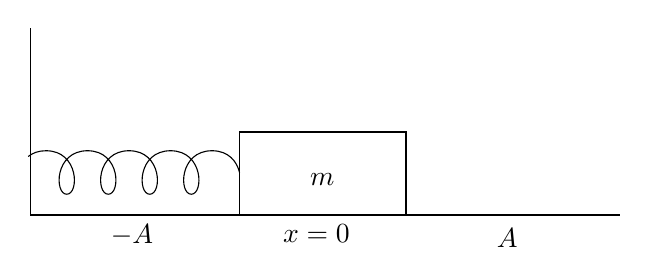
\begin{tikzpicture}[x=0.75pt,y=0.75pt,yscale=-1,xscale=1]
 	\draw   (280.5,131) -- (360.5,131) -- (360.5,171) -- (280.5,171) -- cycle ;
	\draw    (179.5,81) -- (179.5,171) ;
	\draw    (179.5,171) -- (463.5,171) ;
	\draw   (280.31,150.5) .. controls (279.06,145.26) and (275.06,140.02) .. (267.06,140.02) .. controls (251.06,140.02) and (251.06,160.98) .. (257.06,160.98) .. controls (263.06,160.98) and (263.06,140.02) .. (247.06,140.02) .. controls (231.06,140.02) and (231.06,160.98) .. (237.06,160.98) .. controls (243.06,160.98) and (243.06,140.02) .. (227.06,140.02) .. controls (211.06,140.02) and (211.06,160.98) .. (217.06,160.98) .. controls (223.06,160.98) and (223.06,140.02) .. (207.06,140.02) .. controls (191.06,140.02) and (191.06,160.98) .. (197.06,160.98) .. controls (203.06,160.98) and (203.06,140.02) .. (187.06,140.02) .. controls (183.42,140.02) and (180.6,141.11) .. (178.5,142.79) ;

	\draw (313,150) node [anchor=north west][inner sep=0.75pt]    {$m$};
	\draw (300,174.4) node [anchor=north west][inner sep=0.75pt]    {$x=0$};
	\draw (217,174.4) node [anchor=north west][inner sep=0.75pt]    {$-A$};
	\draw (403,176.4) node [anchor=north west][inner sep=0.75pt]    {$A$};
	\end{tikzpicture}
	\caption{Spring in SHM}
\end{figure}

\noindent The mass $m$ has no friction against the surface, and the spring has spring constant $k$. Imposing this system on a circle, we see that the circle is of radius $r = A$. In addition, we can use trigonometry to find that the $x$ coordinate of the block at any point in its path is the same as $A\cos\theta$, where $\theta$ is the angle from the horizontal radius of the circle to the projection of $x$ onto the circle. We also know that $\omega = \theta/t$, as $\theta_o = t_o = 0$. Thus, $\theta = \omega t$. From this, we can derive that $x$, the distance from the equilibrium position is
\[x = A\cos(\omega t),\]
and the derivative of $x$ with respect to time is the velocity, such that
\[v = -A\omega\sin(\omega t)\]
from the chain rule (as $\dv{t} \omega t = \omega$ and $\dv{t} \cos t = -\sin t$). We can also show that
\[a = -A\omega^2\cos(\omega t),\]
since $a = \dv{t} v$. Observe that the farthest possible distance $x$ from equilibrium $x= 0$ is $A$, as $\max a\sin(bt) = a$. Similarly, $\max v = A\omega$ and $\max a = A\omega^2$. The above equations are restated here.
\begin{eqn}
	For an object at the end of a spring oscillating between $x = A$ and $x= -A$,
	\begin{align*}
		x(t) &= A\cos(\omega t) \\
		v(t) &= -A\omega\sin(\omega t) \\
		a(t) &= -A\omega^2\cos(\omega t),
	\end{align*}
	where $t = 0$ at $x = A$.
\end{eqn}
\begin{remark}
	Note that this is subject to where we place $x_o$. For example, setting $t=0$ at $x=0$, where the object moves in the positive $x$ direction, we have
	\[x(t) = A\sin(\omega t),\]
	and the velocity and acceleration follow by differentiating with respect to $t$. 
\end{remark}
Again drawing on the same parallels between circular and harmonic motion, we can define the following values.
\begin{defn}
	The period, $T$, of an object in SHM is the time it takes to complete one cycle in seconds. The frequency, $f$, is the number of cycles an object makes in one second, in Hertz (hz). Finally, the angular frequency $\omega$ of an object is the number of radians it moves in one second, in rad/s.
\end{defn}
Note that this gives us
\[T = \frac{1}{f}.\]
Looking at the graph of $\sin t$, we see that one cycle is equal to $2\pi$ rad. Then, we have
\[\omega = \frac{2\pi}{T},\]
as $\omega = \Delta \theta/\Delta t$, and $t_{2\pi} = T$. Also, we have $\omega = 2\pi f$.

\section{Simple Harmonic Motion \& Pendulums}
In this section, we look at more implications of our study of simple harmonic motion, including pendulums.
\subsection{Harmonic Oscillator with Two Objects}
Examine the following system, similar to the spring we used to study SHM previously, but with an additional block on top.
\begin{figure}[h!]
	\centering
    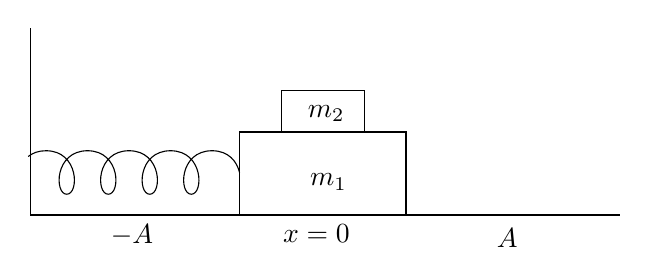
\begin{tikzpicture}[x=0.75pt,y=0.75pt,yscale=-1,xscale=1]
		\draw   (280.5,131) -- (360.5,131) -- (360.5,171) -- (280.5,171) -- cycle ;
		\draw   (300.5,111) -- (340.5,111) -- (340.5,131) -- (300.5,131) -- cycle ;
		\draw    (179.5,81) -- (179.5,171) ;
		\draw    (179.5,171) -- (463.5,171) ;
		\draw   (280.31,150.5) .. controls (279.06,145.26) and (275.06,140.02) .. (267.06,140.02) .. controls (251.06,140.02) and (251.06,160.98) .. (257.06,160.98) .. controls (263.06,160.98) and (263.06,140.02) .. (247.06,140.02) .. controls (231.06,140.02) and (231.06,160.98) .. (237.06,160.98) .. controls (243.06,160.98) and (243.06,140.02) .. (227.06,140.02) .. controls (211.06,140.02) and (211.06,160.98) .. (217.06,160.98) .. controls (223.06,160.98) and (223.06,140.02) .. (207.06,140.02) .. controls (191.06,140.02) and (191.06,160.98) .. (197.06,160.98) .. controls (203.06,160.98) and (203.06,140.02) .. (187.06,140.02) .. controls (183.42,140.02) and (180.6,141.11) .. (178.5,142.79) ;

		\draw (313,150) node [anchor=north west][inner sep=0.75pt]    {$m_1$};
		\draw (312,117) node [anchor=north west][inner sep=0.75pt]    {$m_2$};
		\draw (300,174.4) node [anchor=north west][inner sep=0.75pt]    {$x=0$};
		\draw (217,174.4) node [anchor=north west][inner sep=0.75pt]    {$-A$};
		\draw (403,176.4) node [anchor=north west][inner sep=0.75pt]    {$A$};
	\end{tikzpicture}
	\caption{Spring with two blocks}
\end{figure}

Note that the bottom surface is frictionless, the surface between $m_1$ and $m_2$ has friction so that $m_2$ stays on top of $m_1$.
\begin{question}
	What is the maximum $A$ to which the system can oscillate such that $m_2$ stays at rest on $m_1$?
\end{question}
\begin{solution}
We can start with free-body diagrams. We see that at $x=A$, the acceleration is maximized, meaning that $f_s$ is also maximized. Then,
\[a_{2-\max} = \frac{\mu_sF_n}{m_2} = \mu_sg.\]
This is also equivalent to the maximum acceleration of the system. Thus,
\begin{align*}
	a_{sys-\max} &= \frac{\Sigma F_{sys}}{m_{sys}} \\
	\mu_s g &= \frac{kA}{m1+2},
\end{align*}
as $\Sigma F_{sys} = kx,$ and $x = A$. Then,
\[A_{\max} = \boxed{\frac{(m_1+m_2)\mu_s g}{k}},\]
and we're done.
\end{solution}

\subsection{The Period of a Simple Pendulum}
Observe the pendulum of mass $m$, length $L$, and angle $\theta$ below.\footnote{For this derivation to be successful, $\theta$ must be very small.}
\begin{figure}[h!]
	\centering
    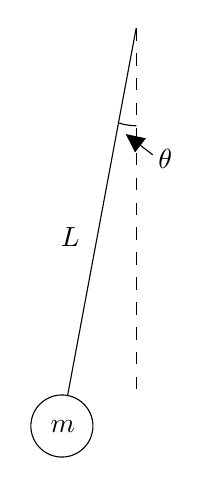
\begin{tikzpicture}[x=0.75pt,y=0.75pt,yscale=-1,xscale=1]
    	\draw  [dash pattern={on 4.5pt off 4.5pt}]  (330.5,50) -- (330.5,230) ;
		\draw    (330.5,50) -- (297.48,226.95) ;
		\draw   (280.03,238.89) .. controls (281.55,230.78) and (289.36,225.43) .. (297.48,226.95) .. controls (305.6,228.46) and (310.95,236.28) .. (309.43,244.39) .. controls (307.91,252.51) and (300.1,257.86) .. (291.98,256.34) .. controls (283.86,254.82) and (278.51,247.01) .. (280.03,238.89) -- cycle ;
		\draw  [draw opacity=0] (330.64,97) .. controls (327.77,96.96) and (325,96.53) .. (322.38,95.74) -- (331,67) -- cycle ;
		\draw   (330.64,97) .. controls (327.77,96.96) and (325,96.53) .. (322.38,95.74) ;
		\draw    (338.5,111) -- (327.88,102.83) ;
		\draw [shift={(325.5,101)}, rotate = 397.57] [fill={rgb, 255:red, 0; green, 0; blue, 0 }  ][line width=0.08]  [draw opacity=0] (8.93,-4.29) -- (0,0) -- (8.93,4.29) -- cycle    ;
		\draw (293,145) node [anchor=north west][inner sep=0.75pt]    {$L$};
		\draw (340,107) node [anchor=north west][inner sep=0.75pt]    {$\theta $};
		\draw (288,238) node [anchor=north west][inner sep=0.75pt]    {$m$};
	\end{tikzpicture}
	\caption{Simple pendulum}
\end{figure}
\begin{question}
	What is the period, $T$, of this pendulum in simple harmonic motion?
\end{question}
\begin{solution}
Recall that in simple harmonic motion, $a = -\omega^2 x$, such that $\omega = \frac{2\pi}{T}$.\footnote{This is from taking the second derivative of $x(t)$, and then observing that $x(t) = A\cos(\omega t)$ and $a(t) = -A\omega^2\cos(\omega t)$, giving us the relation.} From the free-body diagram, observe that the forces acting on $m$ are $mg$ and $F_T$. We can split $mg$ into radial and tangential forces using some basic trigonometry and geometry, giving us that the tangential component is $mg\sin\theta$.

\begin{figure}[h!]
	\centering
    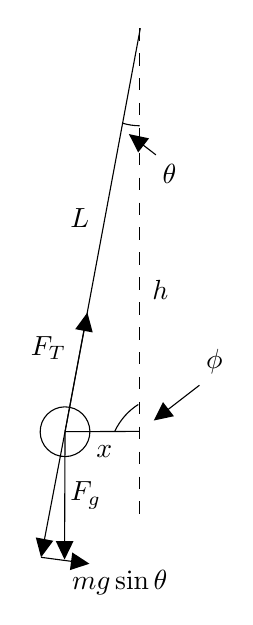
\begin{tikzpicture}[x=0.75pt,y=0.75pt,yscale=-1,xscale=1]
    	\draw  [dash pattern={on 4.5pt off 4.5pt}]  (330.5,50) -- (330.5,290) ;
\draw    (331.01,50) -- (294.73,244.39) ;
\draw   (282.96,242.19) .. controls (284.17,235.69) and (290.43,231.4) .. (296.93,232.62) .. controls (303.44,233.84) and (307.72,240.09) .. (306.51,246.6) .. controls (305.29,253.1) and (299.03,257.39) .. (292.53,256.17) .. controls (286.02,254.95) and (281.74,248.69) .. (282.96,242.19) -- cycle ;
\draw  [draw opacity=0] (330.64,97) .. controls (327.77,96.96) and (325,96.53) .. (322.38,95.74) -- (331,67) -- cycle ; \draw   (330.64,97) .. controls (327.77,96.96) and (325,96.53) .. (322.38,95.74) ;
\draw    (338.5,111) -- (327.88,102.83) ;
\draw [shift={(325.5,101)}, rotate = 397.57] [fill={rgb, 255:red, 0; green, 0; blue, 0 }  ][line width=0.08]  [draw opacity=0] (8.93,-4.29) -- (0,0) -- (8.93,4.29) -- cycle    ;
\draw    (294.73,244.39) -- (330.5,244.24) ;
\draw  [draw opacity=0] (318.74,244.09) .. controls (321.29,238.75) and (325.21,234.3) .. (330.01,231.29) -- (344.75,258.5) -- cycle ; \draw   (318.74,244.09) .. controls (321.29,238.75) and (325.21,234.3) .. (330.01,231.29) ;
\draw    (359.5,222) -- (339.87,237.17) ;
\draw [shift={(337.5,239)}, rotate = 322.31] [fill={rgb, 255:red, 0; green, 0; blue, 0 }  ][line width=0.08]  [draw opacity=0] (8.93,-4.29) -- (0,0) -- (8.93,4.29) -- cycle    ;
\draw    (294.73,244.39) -- (294.51,303) ;
\draw [shift={(294.5,306)}, rotate = 270.21] [fill={rgb, 255:red, 0; green, 0; blue, 0 }  ][line width=0.08]  [draw opacity=0] (8.93,-4.29) -- (0,0) -- (8.93,4.29) -- cycle    ;
\draw    (294.73,244.39) -- (283.73,301.96) ;
\draw [shift={(283.17,304.91)}, rotate = 280.81] [fill={rgb, 255:red, 0; green, 0; blue, 0 }  ][line width=0.08]  [draw opacity=0] (8.93,-4.29) -- (0,0) -- (8.93,4.29) -- cycle    ;
\draw    (283.17,304.91) -- (303.53,307.61) ;
\draw [shift={(306.5,308)}, rotate = 187.55] [fill={rgb, 255:red, 0; green, 0; blue, 0 }  ][line width=0.08]  [draw opacity=0] (8.93,-4.29) -- (0,0) -- (8.93,4.29) -- cycle    ;
\draw    (294.73,244.39) -- (304.95,189.95) ;
\draw [shift={(305.5,187)}, rotate = 460.63] [fill={rgb, 255:red, 0; green, 0; blue, 0 }  ][line width=0.08]  [draw opacity=0] (8.93,-4.29) -- (0,0) -- (8.93,4.29) -- cycle    ;

\draw (296,135.4) node [anchor=north west][inner sep=0.75pt]    {$L$};
\draw (340.5,114.4) node [anchor=north west][inner sep=0.75pt]    {$\theta $};
\draw (361.5,203.4) node [anchor=north west][inner sep=0.75pt]    {$\phi $};
\draw (296,267.4) node [anchor=north west][inner sep=0.75pt]    {$F_{g}$};
\draw (296.84,309.85) node [anchor=north west][inner sep=0.75pt]    {$mg\sin \theta $};
\draw (277,197.4) node [anchor=north west][inner sep=0.75pt]    {$F_{T}$};
\draw (308.51,250) node [anchor=north west][inner sep=0.75pt]    {$x$};
\draw (335.51,170) node [anchor=north west][inner sep=0.75pt]    {$h$};
	\end{tikzpicture}
	\caption{Free body diagram of a pendulum}
\end{figure}

\noindent Then, we have
\begin{align*}
	a &= \frac{\Sigma F}{m} \\
	&= \frac{mg\sin\theta}{m},
\end{align*}
or $a = g\sin\theta$. Now note our assumption that $\theta \simeq 0$. In that case, we can estimate that the arc formed between $m$ and the axis is perpendicular to the axis, meaning that $\phi \simeq 90^{\circ}$. In addition, we have the approximation $h \simeq L$. This yields
\[\tan\theta = \frac{x}{h} \simeq \frac{x}{L} = \sin\theta,\]
or $\tan\theta \simeq \sin\theta$.\footnote{Note that this can also be derived through the approximation $\sin\theta \simeq \theta$ and $\tan\theta \simeq \theta$, also known as the \textit{small angle approximation.}} Thus, $a = g\tan\theta$ and $\tan\theta = \frac{x}{L}$, meaning that $a = -\frac{gx}{L}$. From our original expression, then,
\begin{align*}
	a &= -\frac{gx}{L} \\
	-\omega^2 x &= -\frac{gx}{L} \\
	\omega &= \sqrt{\frac{g}{L}}.
\end{align*}
Finally, since $T\omega = 2\pi$,
\[\boxed{T = 2\pi\sqrt{\frac{L}{g}}},\]
and we're done.
\end{solution}

Again, note that this holds only for small $\theta$, and it's accuracy scales inversely as a function of $\theta$.

\subsection{Horizontal and Vertical Springs.}
Note the following two possible setups for springs.
\begin{figure}[h!]
	\centering
    \begin{tikzpicture}[x=0.75pt,y=0.75pt,yscale=-1,xscale=1]
    	\draw   (341.5,116) -- (410.5,116) -- (410.5,157) -- (341.5,157) -- cycle ;
\draw   (139.5,140.5) .. controls (140.88,134.25) and (145.13,128) .. (153.63,128) .. controls (170.63,128) and (170.63,153) .. (164.63,153) .. controls (158.63,153) and (158.63,128) .. (175.63,128) .. controls (192.63,128) and (192.63,153) .. (186.63,153) .. controls (180.63,153) and (180.63,128) .. (197.63,128) .. controls (214.63,128) and (214.63,153) .. (208.63,153) .. controls (202.63,153) and (202.63,128) .. (219.63,128) .. controls (236.63,128) and (236.63,153) .. (230.63,153) .. controls (224.63,153) and (224.63,128) .. (241.63,128) .. controls (258.63,128) and (258.63,153) .. (252.63,153) .. controls (246.63,153) and (246.63,128) .. (263.63,128) .. controls (280.63,128) and (280.63,153) .. (274.63,153) .. controls (268.63,153) and (268.63,128) .. (285.63,128) .. controls (302.63,128) and (302.63,153) .. (296.63,153) .. controls (290.63,153) and (290.63,128) .. (307.63,128) .. controls (314.35,128) and (318.41,131.91) .. (320.5,136.64) ;
\draw    (320.5,137) -- (341.5,137) ;
\draw    (138.5,157) -- (481.5,157) ;
\draw    (138.5,60) -- (138.5,157) ;
\draw    (322,104.5) -- (430,104.5) ;
\draw [shift={(433,104.5)}, rotate = 180] [fill={rgb, 255:red, 0; green, 0; blue, 0 }  ][line width=0.08]  [draw opacity=0] (8.93,-4.29) -- (0,0) -- (8.93,4.29) -- cycle    ;
\draw [shift={(319,104.5)}, rotate = 0] [fill={rgb, 255:red, 0; green, 0; blue, 0 }  ][line width=0.08]  [draw opacity=0] (8.93,-4.29) -- (0,0) -- (8.93,4.29) -- cycle    ;
\draw   (312.52,170.09) .. controls (318.78,171.44) and (325.04,175.68) .. (325.06,184.18) .. controls (325.11,201.18) and (300.11,201.25) .. (300.09,195.25) .. controls (300.08,189.25) and (325.08,189.18) .. (325.12,206.18) .. controls (325.17,223.18) and (300.17,223.25) .. (300.16,217.25) .. controls (300.14,211.25) and (325.14,211.18) .. (325.19,228.18) .. controls (325.23,245.18) and (300.23,245.25) .. (300.22,239.25) .. controls (300.2,233.25) and (325.2,233.18) .. (325.25,250.18) .. controls (325.3,267.18) and (300.3,267.25) .. (300.28,261.25) .. controls (300.26,255.25) and (325.26,255.18) .. (325.31,272.18) .. controls (325.36,289.18) and (300.36,289.25) .. (300.34,283.25) .. controls (300.32,277.25) and (325.32,277.18) .. (325.37,294.18) .. controls (325.42,311.18) and (300.42,311.25) .. (300.4,305.25) .. controls (300.38,299.25) and (325.38,299.18) .. (325.43,316.18) .. controls (325.48,333.18) and (300.48,333.25) .. (300.46,327.25) .. controls (300.45,321.25) and (325.45,321.18) .. (325.49,338.18) .. controls (325.51,344.9) and (321.61,348.98) .. (316.89,351.08) ;
\draw    (317.53,351.08) -- (317.59,372.08) ;
\draw    (269.03,339.49) -- (269.34,447.49) ;
\draw [shift={(269.34,450.49)}, rotate = 269.84000000000003] [fill={rgb, 255:red, 0; green, 0; blue, 0 }  ][line width=0.08]  [draw opacity=0] (8.93,-4.29) -- (0,0) -- (8.93,4.29) -- cycle    ;
\draw [shift={(269.03,336.49)}, rotate = 89.84] [fill={rgb, 255:red, 0; green, 0; blue, 0 }  ][line width=0.08]  [draw opacity=0] (8.93,-4.29) -- (0,0) -- (8.93,4.29) -- cycle    ;
\draw   (283.5,372) -- (352.5,372) -- (352.5,413) -- (283.5,413) -- cycle ;
\draw    (138.5,170) -- (482.5,170) ;
	\end{tikzpicture}
	\caption{Orientations of a spring}
\end{figure}

\medskip

\begin{question}
	What is the difference between the vertical spring and horizontal spring?
\end{question}
Interestingly, we can ignore the force of gravity in the vertical spring, meaning that there is effectively no difference in our analysis. Observe that in the vertical case, once the object is attached extending the spring, there is a restoring force $F = kx_o$, where $x_o$ is the amount of distance the spring was extended. From a force perspective, we can see that
\[\Sigma F_y = kx_o - mg = 0,\]
so $mg = kx_o$. Now suppose that we stretch this spring further by distance $x$. Then, the forces acting upon it are $F = k(x_o+x)$ and $mg$. Therefore,
\begin{align*}
	\Sigma F_y &= k(x+x_o) -mg \\
	&= kx + kx_o - mg \\
	&= kx + mg - mg,
\end{align*}
so $\Sigma F_y = kx$. In the case of the horizontal spring, we see that $\Sigma F_x = kx$, meaning that there is no difference.


\bigskip\bigskip

\begin{center}
    The End.
\end{center}


\newpage

\bigskip\bigskip

\begin{center}
    The End.
\end{center}


\newpage

\part{Mathematical Appendix}
This section contains a brief review of the calculus and other non-pre-calculus math used in the notes and the course.

\section{Differential Calculus Review}
The derivative of a function $f(x):\RR\to\RR$ is given by
\begin{equation}
    f'(x) = \dv{x} f(x) = \lim_{h\to 0}\frac{f(x+h) - f(x)}{h}.
\end{equation}
We can use  derivative rules when calculating derivatives of functions:
\begin{align}
    \dv{x} Cf(x) &= C\dv{x} f(x) \\
    \dv{x} x^n &= nx^{n-1} \\
    \dv{x} (f(x) + g(x)) &= f'(x) + g'(x) \\
    \dv{x} (f(x) \cdot g(x)) &= f'(x)g(x) + f(x)g'(x) \\
    \dv{x} \p{\frac{f(x)}{g(x)}} &= \frac{f'(x)g(x) - f(x)g'(x)}{(g(x))^2} \\
    \dv{x} f(g(x)) &= f'(g(x))g'(x).
\end{align}
Other common derivatives:
\begin{align}
    \dv{x} e^{x} &= e^x \\
    \dv{x} \ln(x) &= \frac{1}{x} \\
    \dv{x} \sin(x) &= \cos(x) \\
    \dv{x} \cos(x) &= \sin(x) \\
    \dv{x} \tan(x) &= \sec^2(x).
\end{align}
Most other derivatives can be computed through trivial application of the chain, product, and quotient rules. Additionally, TI-84 calculators can compute derivatives at a point $x$ using the function \texttt{nDeriv(function, variable, value)}.

\section{Integral Calculus Review}
The indefinite integral of a function $f(x):\RR\to\RR$ is the function $F(x)$ such that
\begin{equation}
    f(x) = F'(x),
\end{equation}
which is written as
\begin{equation}
    \int f(x) = F(x).
\end{equation}
The definite integral of $f$ is defined as
\begin{equation}
    \int_a^b f(x) = \lim_{n \to\infty}\sum_{i=1}^{\infty} \frac{b-a}{n}\cdot f(x_i).
\end{equation}
If $F(x)$ is an antiderivative of $f(x)$, the Fundamental Theorem of Calculus states
\begin{equation}
    \int_a^b f(x) = F(a) - F(b).
\end{equation}
Common integral rules are effectively the rules described in the previous section, but in reverse.

One common method of evaluating an integral, often called the ``opposite of the chain rule,'' is $u$-substitution, which is particularly prevalent in solving differential equations (e.g. for the behavior of resistive forces, capacitors, and inductors). For $u$-substitution, if a function $f(x)$ can be expressed as $g(h(x))$ for functions $g$ and $h$, $u$-substitution allows us to substitute $u = h(x)$, such that we have $\dd u = h'(x) \dd x$. For example,
\[\int e^{\sin x}\cos x \dd x\]
can be written as
\[\int e^u\dd u,\]
where $u = \sin x$ and $\dd u = \cos x\dd x$. This integral is much simpler to evaluate, resolving to
\[e^{u} + C = e^{\sin x} + C.\]

Another common method of integration is integration by parts, which is effectively the opposite of the product rule. It is stated as
\begin{equation}
    \int u\dd v = uv - \int v\dd u.
\end{equation}
For example, the above integral of $e^{\sin x} \cos x$ can be expressed as
\[e^{\sin x}\sin x - \int \sin x\cos x e^{\sin x} \dd x.\]

\section{Vectors and Vector Calculus}
A vector is a quantity in vector space with both magnitude and direction. Vectors can be written in two forms: component form or unit vector form, or with their magnitude and angle. In component form, a vector $\vec{v}$ is written as \[\vec{v} = \bvec{v_x, v_y, v_z}.\] In unit vector form, this is expressed as \[\vec{v} = v_x\vu{\imath} + v_y\vu{\jmath} + v_z\vu{k},\] where $\vu{\imath}, \vu{\jmath},$ and $\vu{k}$ are vectors with magnitude 1.  The magnitude of a vector is given by $\sqrt{v_x^2+v_y^2+v_z^2}$, and is notated $|\vec{v}|$ (or $||\vec{v}||$).

Basic vector operations are very simple. To add two vectors, we add their components, such that $\vec{u} + \vec{v} = \bvec{u_x + v_x, u_y + v_y, u_z + v_z}$. The same is true of subtraction. There are two types of products between vectors: the \textbf{dot product} (or scalar product), and the \textbf{cross product} (or vector product). The dot product produces a scalar, such that
\begin{equation}
    \vec{u} \cdot \vec{v} = u_xv_x + u_yv_y + u_zv_z = |u||v|\cost
\end{equation}
Contrastingly, the cross product produces a vector, given by
\begin{equation}
    \vec{u} \times \vec{v} = \begin{vmatrix}
        \vu{\imath} & \vu{\jmath} & \vu{k} \\
        u_x & u_y & u_z \\
        v_x & v_y & v_z
    \end{vmatrix},
\end{equation}
or the determinant of the matrix. The magnitude of the cross product is given by $|u||v|\sint$, where $\theta$ is the angle between the vectors.

Calculus with vectors is relatively simple. The derivative of a vector valued function $\vec{v}(t) = \bvec{v_x(t), v_y(t), v_z(t)}$ is simply
\begin{equation}
    \dv{t}\vec{v}(t) = \bvec{v'_x(t), v'_y(t), v'_z(t)}
\end{equation}
Similarly, the integral of a vector valued function is
\begin{equation}
    \int \vec{v}(t) \dd t = \bvec{\int v_x(t)\dd t, \int v_y(t)\dd t, \int v_z(t)\dd t}.
\end{equation}

Additionally, we use \textbf{vector fields}, written in boldface, to describe the magnitude and direction of a vector at a given point in space. Figure~\ref{vectorfieldexample} is an example of a vector field. In physics, the three most common vector fields are the gravitational field $\mathbf{g}$, the electric field $\mathbf{E}$, and the magnetic field $\mathbf{B}$. Any vector operation can occur between a vector and a vector field, with the effect of that operation occurring on each vector in the field.

\begin{figure}[t!]\label{vectorfieldexample}
    \centering
    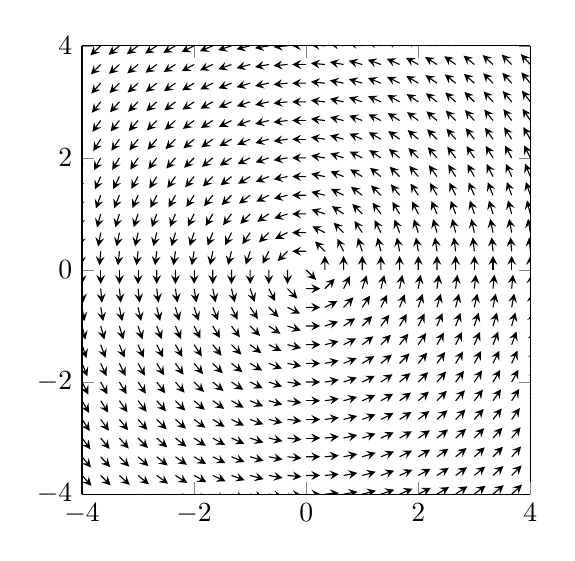
\begin{tikzpicture}
    \begin{axis}[
        xmin = -4, xmax = 4,
        ymin = -4, ymax = 4,
        zmin = 0, zmax = 1,
        axis equal image,
        view = {0}{90},
    ]
        \addplot3[
            quiver = {
                u = {-y/sqrt(x^2+y^2)},
                v = {x/sqrt(x^2+y^2)},
                scale arrows = 0.25,
            },
            -stealth,
            domain = -4:4,
            domain y = -4:4,
        ] {0};
    \end{axis}
    \end{tikzpicture}
\caption{An example vector field}
\end{figure}

With vector fields, two additional types of integrals arise in the AP Physics curriculum. The first is the \textbf{closed surface integral}, which appears in both of Gauss's laws. It is defined as
\begin{equation}
    \oint_A \mathbf{F} \cdot \dd A,
\end{equation}
where $\mathbf{F}$ is a vector field, and $\dd \vec{A}$ represents the normal through a small area. For the most part, these integrals quickly resolve to $|F|A$, where $A$ is the surface area, as the dot product will trivially collapse since $\theta = 90\degr$. Additionally, there is the \textbf{closed loop integral}, which is similar:
\begin{equation}
    \oint_{\ell} \mathbf{F} \cdot \dd\vec{\ell},
\end{equation}
where $\vec{\ell}$ is the normal through a small length. This appears in Ampere's law, and typically resolves to $|F|L$, where $L$ is the length of the loop.
\end{document}